\documentclass[journal]{IEEEtran}
% \documentclass[journal,12pt,onecolumn,draftclsnofoot]{IEEEtran}

\usepackage[table]{xcolor}
\usepackage{adjustbox}
\usepackage{algorithm}
\usepackage{algpseudocode}
\usepackage{amsfonts}
\usepackage{amsmath}
\usepackage{amssymb}
\usepackage{amsthm}
\usepackage{bookmark}
\usepackage{booktabs}
\usepackage[makeroom]{cancel}
\usepackage[american]{circuitikz}
\usepackage{cite}
\usepackage{fixmath}
\usepackage[acronym]{glossaries-extra}
\usepackage{hyperref}
\usepackage{import}
\usepackage{mathtools}
\usepackage{microtype}
\usepackage[short]{optidef}
\usepackage{pgfplots}
\usepackage{ragged2e}
\usepackage[subtle]{savetrees}
\usepackage{siunitx}
\usepackage{stfloats}
\usepackage[caption=false,font=footnotesize,subrefformat=parens,labelformat=parens]{subfig}
\usepackage{tabularx}
\usepackage{tikz}
\usepackage{graphicx}
\usepackage{epstopdf}
% \usepackage{cleveref}

% page limit hacks
% \usepackage{setspace}
% ! \usepackage[top=1cm, bottom=1cm, left=1cm, right=1cm]{geometry}
% \abovedisplayskip=1mm
% \belowdisplayskip=1mm
% \abovedisplayshortskip=1mm
% \belowdisplayshortskip=1mm
% \setlength{\jot}{0.1mm}
% \setlength{\floatsep}{1mm}
% \setlength{\textfloatsep}{1mm}
% \setlength{\intextsep}{1mm}
% \setlength{\skip\footins}{2mm}


% amsthm
\newtheorem{proposition}{Proposition}
\newtheorem{remark}{Remark}
\newtheorem{lemma}{Lemma}

% PGF/TikZ
\usetikzlibrary{arrows,calc,matrix,patterns,plotmarks,positioning,shapes}
\usetikzlibrary{decorations.pathmorphing,decorations.pathreplacing,decorations.shapes,shapes.geometric}
\usepgfplotslibrary{groupplots,patchplots}
\pgfplotsset{compat=newest}

% tabularx, ragged2e
\newcolumntype{L}{>{\RaggedRight}X}
\newcolumntype{C}{>{\centering\arraybackslash}X}
\renewcommand\tabularxcolumn[1]{m{#1}}

% algpseudocode
\makeatletter
\renewcommand{\fnum@algorithm}{\fname@algorithm{} \thealgorithm:}
\newcommand\setalgorithmcaptionfont[1]{%
	\let\my@floatc@ruled\floatc@ruled          % save \floatc@ruled
	\def\floatc@ruled{%
		\global\let\floatc@ruled\my@floatc@ruled % restore \floatc@ruled
		#1\floatc@ruled}}
\makeatother

\algrenewcommand{\algorithmicrequire}{\textbf{Input:}}
\algrenewcommand{\algorithmicensure}{\textbf{Output:}}
\algrenewcommand{\algorithmicwhile}{\textbf{While}}
\algrenewcommand{\algorithmicend}{\textbf{End}}
\algrenewcommand{\algorithmicrepeat}{\textbf{Repeat}}
\algrenewcommand{\algorithmicuntil}{\textbf{Until}}
\algrenewcommand{\algorithmicfor}{\textbf{For}}
\algrenewcommand{\algorithmicif}{\textbf{If}}
\algrenewcommand{\algorithmicelse}{\textbf{Else}}
\algrenewcommand{\algorithmicdo}{}
\algrenewcommand{\algorithmicthen}{}
\algnewcommand{\Initialize}[1]{%
	\State \textbf{Initialize }{#1}
}

% optidef
\DeclareDocumentEnvironment{customopti}{D||{\defaultProblemFormat} O{\defaultConstraintFormat} D<>{} m m m m m}{%
	\ifthenelse{\equal{#3}{b}}{%
		\ifthenelse{\equal{#1}{s}}%
		% Short version problem
		{\setFormatShort{#4}{#5}\BaseMiniStar{#2}{#5}{#6}{#8}{#4}{#3}}%
		% Long version problem
		{\setFormatLong{#4}{#5}\BaseMiniStar{#2}{#5}{#6}{#8}{#4}{#3}}%
	}{%
		\ifthenelse{\equal{#1}{s}}%
		% Short version problem
		{\setFormatShort{#4}{#5}\BaseMini{#2}{#5}{#6}{#7}{#8}{#4}}%
		% Long version problem
		{\setFormatLong{#4}{#5}\BaseMini{#2}{#5}{#6}{#7}{#8}{#4}}%
	}%
}%
{\endBaseMini\toggletrue{bodyCon}}

\DeclareDocumentEnvironment{customopti*}{D||{\defaultProblemFormat} O{\defaultConstraintFormat} D<>{} m m m m m}{%
	\ifthenelse{\equal{#1}{s}}%
	% Short version problem
	{\setFormatShort{#4}{#5}\BaseMiniStar{#2}{#5}{#6}{#8}{#4}{#3}}%
	% Long version problem
	{\setFormatLong{#4}{#5}\BaseMiniStar{#2}{#5}{#6}{#8}{#4}{#3}}%
}{\endBaseMiniStar\toggletrue{bodyCon}}

\DeclareDocumentEnvironment{customopti!}{D||{\defaultProblemFormat} O{\defaultConstraintFormat} D<>{} m m m m m}{%
	\ifthenelse{\equal{#1}{s}}%
	% Short version problem
	{\setFormatShort{#4}{#5}\BaseMiniExclam{#2}{#5}{#6}{#7}{#8}{#4}{#3}}%
	% Long version problem
	{\setFormatLong{#4}{#5}\BaseMiniExclam{#2}{#5}{#6}{#7}{#8}{#4}{#3}}%
}{\endBaseMiniExclam\toggletrue{bodyCon}}

% glossaries-extra
\glsdisablehyper
\setabbreviationstyle[acronym]{long-short}
\newacronym{ao}{AO}{Alternating Optimization}
\newacronym{bd}{BD}{Beyond-Diagonal}
\newacronym{bcd}{BCD}{Block Coordinate Descent}
\newacronym{dof}{DoF}{Degree of Freedom}
\newacronym{siso}{SISO}{Single-Input Single-Output}
\newacronym{miso}{MISO}{Multiple-Input Single-Output}
\newacronym{mimo}{MIMO}{Multiple-Input Multiple-Output}
\newacronym{rcg}{RCG}{Riemannian Conjugate Gradient}
\newacronym{ris}{RIS}{Reconfigurable Intelligent Surface}
\newacronym{pc}{PC}{Point-to-point Channel}
\newacronym{ic}{IC}{Interference Channel}
\newacronym{snr}{SNR}{Signal-to-Noise Ratio}
\newacronym{wsr}{WSR}{Weighted Sum-Rate}
\newacronym{svd}{SVD}{Singular Value Decomposition}
\newacronym{mmse}{MMSE}{Minimum Mean-Square Error}
\newacronym{wmmse}{WMMSE}{Weighted \gls{mmse}}
\newacronym{mse}{MSE}{Mean-Square Error}
\newacronym{los}{LoS}{Line-of-Sight}
\newacronym{csi}{CSI}{Channel State Information}
\newacronym{cscg}{CSCG}{Circularly Symmetric Complex Gaussian}


\begin{document}
\title{Channel Shaping Using Reconfigurable Intelligent Surfaces: From Diagonal to Beyond}
\author{
	\IEEEauthorblockN{
		Yang~Zhao,~\IEEEmembership{Member,~IEEE,}
		Hongyu~Li,~\IEEEmembership{Graduate Student Member,~IEEE,}\\
		Massimo~Franceschetti,~\IEEEmembership{Fellow,~IEEE,}
		and~Bruno~Clerckx,~\IEEEmembership{Fellow,~IEEE}
	}
	% \thanks{
	% 	The authors are with the Department of Electrical and Electronic Engineering, Imperial College London, London SW7 2AZ, U.K. (e-mail: \{yang.zhao18, b.clerckx\}@imperial.ac.uk).
	% 	B. Clerckx is also with Silicon Austria Labs (SAL), Graz A-8010, Austria.
	% }
}
\maketitle

\begin{abstract}
	This paper investigates how a passive \gls{ris} can reshape the \gls{mimo} point-to-point channel in terms of singular values.
	We depart from the widely-adapted diagonal phase shift model to a general \gls{bd} architecture, which provides superior shaping capability thanks to in-group connections between elements.
	An efficient \gls{rcg} algorithm is tailored for smooth optimization problems of asymmetric \gls{bd}-\gls{ris} with arbitrary group size, then invoked for the Pareto frontier of channel singular values.
	To understand the gain from off-diagonal entries, we also derive analytical singular value bounds in \gls{los} and fully-connected scenarios.
	As a side product, we tackle \gls{mimo} rate maximization problem by alternating between active beamformer (eigenmode transmission) and passive beamformer (\gls{rcg} algorithm) until convergence.
	A low-complexity suboptimal solution based on channel shaping is also proposed, where the decoupled problem is formulated as channel power maximization and solved in closed form iteratively.
	% We then show how channel shaping decouples the design and amounts to a low-complexity suboptimal solution.
	% A low-complexity suboptimal solution decoupling both blocks is also proposed, where the channel shaping subproblem is formulated as channel power maximization and solved in closed form iteratively.
	Theoretical analysis and numerical evaluation reveal that the shaping advantage of \gls{bd}-\gls{ris} increases with group size and \gls{mimo} dimensions, stemming from stronger subchannel rearrangement and subspace alignment capabilities.
\end{abstract}

\begin{IEEEkeywords}
	Reconfigurable intelligent surface, multi-input multi-output, manifold optimization, singular value control, rate maximization.
\end{IEEEkeywords}

\glsresetall

\begin{section}{Introduction}
	% The quest for reliable, high-speed, and ubiquitous wireless connectivity has been long-standing since Marconi's illuminating radio in 1895.
	% Great successes have been made at transmitter and receiver sides over the past century, and the society is unprecedentedly close to the Shannon limit \cite{Shannon1948}.
	Today we are witnessing a paradigm shift from connectivity to intelligence, where the wireless environment is no longer a chaotic medium but a conscious agent that serves on demand.
	This is empowered by the recent advances in \gls{ris}, a real-time programmable metasurface of numerous non-resonant sub-wavelength scattering elements.
	It can manipulate the amplitude, phase, frequency, and polarization of the scattered waves \cite{Basar2019} with a higher energy efficiency, lower cost, lighter footprint, and greater scalability than relays.
	Using \gls{ris} for {passive beamforming} has attracted significant interest in wireless communication \cite{Wu2019,Wu2020c,Yang2020,Zheng2021}, backscatter \cite{Jia2020,Liang2022}, sensing \cite{Liu2022a,Hua2023}, and power transfer literature \cite{Wu2021d,Feng2022,Zhao2022}, reporting a second-order array gain and fourth-order power scaling law (with proper waveform).
	On the other hand, \gls{ris} also enables {backscatter modulation} by dynamically switching between different patterns, as already investigated \cite{Karasik2020,Basar2020,Zhao2022a} and prototyped \cite{Tang2019a,Dai2020a}.
	Despite fruitful outcomes, one critical unanswered question is the {channel shaping} capability: \emph{To what extent can a passive \gls{ris} reshape the wireless channel?}

	The answer indeed depends on the hardware architecture and scattering model.
	In conventional (a.k.a. diagonal) \gls{ris}, each scattering element is tuned by a dedicated impedance and acts as an \emph{individual} phase shifter \cite{Wu2020}.
	The concept is generalized to \gls{bd}-\gls{ris} \cite{Shen2020a,Li2023b} which groups adjacent elements using passive components.
	This allows \emph{cooperative} scattering --- wave impinging on one element can propagate within the circuit and depart partially from any element in the same group.
	\gls{bd}-\gls{ris} can thus control both amplitude and phase of the reflected wave, generalizing the scattering matrix from diagonal with unit-magnitude entries to block diagonal with  unitary blocks.
	Its benefit has been recently shown in receive power maximization \cite{Nerini2023,Santamaria2023,Fang2023,Nerini2023a}, transmit power minimization \cite{Zhou2023}, and rate maximization \cite{Zhou2023,Nerini2023a,Li2023d,Bartoli2023,Li2023c}.
	Practical issues such as channel estimation \cite{Li2023e} and mutual coupling \cite{Li2023f} have also been investigated.
	Therefore, \gls{bd}-\gls{ris} is envisioned as the next generation channel shaper with stronger signal processing flexibility \cite{Li2023g}.

	% Attempts to characterize the channel shaping capability can be classified into \emph{singular value centric} and \emph{power centric} methods.
	% Channel shaping is different from passive beamforming as it seeks to modify the inherent properties of the channel itself, allowing one to decouple \gls{ris} and transceiver design.
	Channel shaping is different from passive beamforming as it seeks to modify the inherent properties of the channel itself.
	This allows one to decouple the \gls{ris}-transceiver design and explore the fundamental limits of channel manipulation.
	For example, diagonal \gls{ris} has been proved useful for improving channel power \cite{Ning2020}, degree of freedom \cite{Ozdogan2020,Li2023h}, condition number \cite{Zheng2022,Huang2023}, and effective rank \cite{ElMossallamy2021,Meng2023} in \gls{mimo}.
	In contrast, \gls{bd}-\gls{ris} can provide a higher channel power but existing results are limited to \gls{siso}\footnote{In terms of channel shaping, single-stream \gls{mimo} with given precoder and combiner \cite{Nerini2023} is equivalent to \gls{siso}.}. \cite{Nerini2023} and \gls{miso} \cite{Santamaria2023}.
	While these studies offer promising glimpses into the channel shaping potential, a comprehensive understanding of the capabilities and limitations is desired, and a universal design framework is missing.
	This paper aims to answer the channel shaping question through theoretical analysis and numerical optimization.
	The contributions are summarized below.

	First, we quantify the capability of a \gls{bd}-\gls{ris} to reshape the \gls{mimo} point-to-point channel in terms of singular values.
	The \emph{Pareto frontiers} are characterized by optimizing the {weighted sum of singular values}, where the weights can be positive, zero, or negative.
	% This generalizes most singular value metrics and provides a powerful design framework.
	The resulting singular value region generalizes most relevant metrics and provides an intuitive channel shaping benchmark.
	We then discuss some analytical singular value bounds in \gls{los} and fully-connected scenarios, which help to demystify the gain from off-diagonal entries.
	This is the first paper to answer the channel shaping question and highlight the \gls{bd}-\gls{ris} gain from a Pareto perspective.

	Second, we propose a \gls{rcg} algorithm adapted from \cite{Abrudan2008,Abrudan2009} for smooth optimization problems of asymmetric \gls{bd}-\gls{ris} with arbitrary group size.
	Specifically, block-wise update is performed along the geodesics\footnote{A geodesic refers to the shortest path between two points in a Riemannian manifold.} of the Stiefel manifold, which are expressed compactly by the exponential map \cite{Edelman1998}.
	It features lower complexity and faster convergence than general manifold optimization \cite{Absil2009,Pan2022d}, and solves the Pareto singular value problem.
	This is the first paper to tailor an efficient optimization framework for asymmetric \gls{bd}-\gls{ris}.

	Third, we tackle \gls{bd}-\gls{ris} \gls{mimo} rate maximization with two solutions: a local-optimal approach through \gls{ao} and a low-complexity approach over channel shaping.
	The former updates active and passive beamformers by eigenmode transmission and \gls{rcg} algorithm, respectively.
	The latter suboptimally decouples both blocks, recasts the shaping problem as channel power maximization, and solves it iteratively in closed form.
	Interestingly, the gap in between vanishes as \gls{bd}-\gls{ris} evolves from diagonal (single-connected) to unitary (fully-connected).
	It suggests channel shaping offers a promising low-complexity solution for joint \gls{ris}-transceiver designs.

	% Third, we propose a closed-form iterative algorithm for power centric channel shaping problems.
	% The idea is to successively approximate the quadratic objective by a sequence of affines and solve the local problems by \gls{svd}.
	% Case studies are conducted for channel power maximization in \gls{pc} and leakage interference minimization in \gls{ic}.

	Fourth, extensive simulations reveal that the performance gain from \gls{bd}-\gls{ris} increases with group size and \gls{mimo} dimensions.
	In terms of channel power, fully-connected \gls{bd}-\gls{ris} boosts up to 62\%, 312\%, 537\% over single-connected in $1 \times 1$, $4 \times 4$, $16 \times 16$ \gls{mimo} under independent Rayleigh fading, respectively.
	The superiority stems from stronger \emph{subchannel rearrangement} and \emph{subspace alignment} capabilities empowered by in-group cooperation.
	It emphasizes the importance of using \gls{bd}-\gls{ris} in large-scale \gls{mimo} systems.


	\emph{Notation:}
	Italic, bold lower-case, and bold upper-case letters indicate scalars, vectors and matrices, respectively.
	$\jmath$ denotes the imaginary unit.
	$\mathbb{C}$ represents the set of complex numbers.
	$\mathbb{U}^{n \times n}$ denotes the set of $n \times n$ unitary matrices.
	$\mathbf{0}$ and $\mathbf{I}$ are the all-zero and identity matrices with appropriate size, respectively.
	$\mathrm{tr}(\cdot)$ and $\det(\cdot)$ evaluates the trace and determinant of a square matrix, respectively.
	$\mathrm{diag}(\cdot)$ constructs a square matrix with arguments on the main diagonal and zeros elsewhere.
	$\mathrm{sv}(\cdot)$ returns the singular value vector.
	$\sigma_n(\cdot)$ and $\lambda_n(\cdot)$ is the $n$-th largest singular value and eigenvalue, respectively.
	% $\boldsymbol{\sigma}(\cdot)$ and $\boldsymbol{\lambda}(\cdot)$ are the corresponding vectors.
	$(\cdot)^*$, $(\cdot)^\mathsf{T}$, $(\cdot)^\mathsf{H}$, $(\cdot)^{(r)}$, $(\cdot)^{\star}$ denote the conjugate, transpose, conjugate transpose (Hermitian), $r$-th iterated point, and final solution, respectively.
	$\lvert \cdot \rvert$ denotes the absolute value.
	$\lVert \cdot \rVert _p$ means the $p$-norm and $\lVert \cdot \rVert$ suggests $p = 2$.
	$\lVert \cdot \rVert _\mathrm{F}$ represents the Frobenius norm.
	$\sim$ means ``distributed as''.
	$\mathcal{CN}(\mathbf{0}, \mathbf{\Sigma})$ is the multivariate \gls{cscg} distribution with mean $\mathbf{0}$ and covariance $\mathbf{\Sigma}$.
\end{section}

\begin{section}{\gls{bd}-\gls{ris} Model}
	Consider a \gls{bd}-\gls{ris} aided point-to-point \gls{mimo} system with $N_\mathrm{T}$, $N_\mathrm{S}$, $N_\mathrm{R}$ transmit, scatter, and receive antennas, respectively.
	This configuration is denoted as $N_\mathrm{T} \times N_\mathrm{S} \times N_\mathrm{R}$.
	The \gls{bd}-\gls{ris} is modeled as an $N_\mathrm{S}$-port network \cite{Ivrlac2010} that further divides into $G$ individual groups.
	Each group contains $L \triangleq N_\mathrm{S} / G$ elements interconnected by real-time reconfigurable components \cite{Shen2020a}.
	To simplify the analysis, we assume there are no mutual coupling and the in-group connections can be lossless and asymmetric\footnote{While symmetric impedance network is often considered in the literature \cite{Shen2020a,Nerini2023,Santamaria2023,Fang2023,Nerini2023a,Zhou2023,Li2023d,Bartoli2023}, asymmetric passive components (e.g., ring hybrids and branch-line hybrids) may also be reconfigured in real time \cite{Ahn2006}. Asymmetric \gls{bd}-\gls{ris} has been discussed in \cite{Li2023b,Li2023c,Bartoli2023}.}.
	The overall scattering matrix is thus block diagonal $\mathbf{\Theta} = \mathrm{diag}(\mathbf{\Theta}_1,\ldots,\mathbf{\Theta}_G) \in \mathbb{U}^{N_\mathrm{S} \times N_\mathrm{S}}$, where $\mathbf{\Theta}_g \in \mathbb{U}^{L \times L}$ is a unitary matrix corresponding to group $g \in \mathcal{G} \triangleq \{1,\ldots,G\}$.
	Let $\mathbf{H}_\mathrm{D} \in \mathbb{C}^{N_\mathrm{R} \times N_\mathrm{T}}$, $\mathbf{H}_\mathrm{F} \in \mathbb{C}^{N_\mathrm{S} \times N_\mathrm{T}}$, $\mathbf{H}_\mathrm{B} \in \mathbb{C}^{N_\mathrm{R} \times N_\mathrm{S}}$ denote the direct (transmitter-receiver), forward (transmitter-\gls{ris}), and backward (\gls{ris}-receiver) channels, respectively.
	The equivalent channel is
	\begin{equation}
		\mathbf{H} = \mathbf{H}_\mathrm{D} + \mathbf{H}_\mathrm{B} \mathbf{\Theta} \mathbf{H}_\mathrm{F} = \mathbf{H}_\mathrm{D} + \sum_g \mathbf{H}_{\mathrm{B},g} \mathbf{\Theta}_g \mathbf{H}_{\mathrm{F},g},
		\label{eq:channel_equivalent}
	\end{equation}
	where $\mathbf{H}_{\mathrm{B},g} \in \mathbb{C}^{N_\mathrm{R} \times L}$ and $\mathbf{H}_{\mathrm{F},g} \in \mathbb{C}^{L \times N_\mathrm{T}}$ are the backward and forward channels of \gls{ris} group $g$, respectively.
	\begin{remark}
		\gls{bd}-\gls{ris} reduces to diagonal \gls{ris} and unitary \gls{ris} with group size 1 and $N_\mathrm{S}$, respectively.
	\end{remark}
	\begin{remark}
		Individual forward and backward \gls{csi} are required for \gls{bd}-\gls{ris} designs.
		This is different from diagonal \gls{ris} where estimating their product is usually sufficient.
		% Later we will show the potential benefits from the \gls{csi} overhead.
	\end{remark}
\end{section}

\begin{section}{Channel Singular Value Redistribution}
	\begin{subsection}{A Toy Example}
		We first illustrate the channel shaping capabilities of different \gls{ris} by a toy example.
		% We first use a toy example to illustrate that \gls{bd}-\gls{ris} can provide a wider dynamic range of channel singular values.
		Consider a $2 \times 2 \times 2$ setup where the direct link is blocked.
		The diagonal \gls{ris} is modeled by $\mathbf{\Theta}_\mathrm{D} = \mathrm{diag}(e^{\jmath \theta_1}, e^{\jmath \theta_2})$ while the unitary \gls{bd}-\gls{ris} has 4 independent angular parameters
		\begin{equation}
			\mathbf{\Theta}_\mathrm{U} = e^{\jmath \phi} \begin{bmatrix}
				e^{\jmath \alpha} \cos \psi  & e^{\jmath \beta} \sin \psi   \\
				-e^{-\jmath \beta} \sin \psi & e^{-\jmath \alpha} \cos \psi
			\end{bmatrix}.
		\end{equation}
		In particular, $\phi$ has no impact on the singular value because $\mathrm{sv}(e^{\jmath \phi} \mathbf{A}) = \mathrm{sv}(\mathbf{A})$.
		We also enforce symmetry by $\beta = \pi / 2$ such that both architectures have the same number of angular parameters.
		\begin{figure}
			\centering
			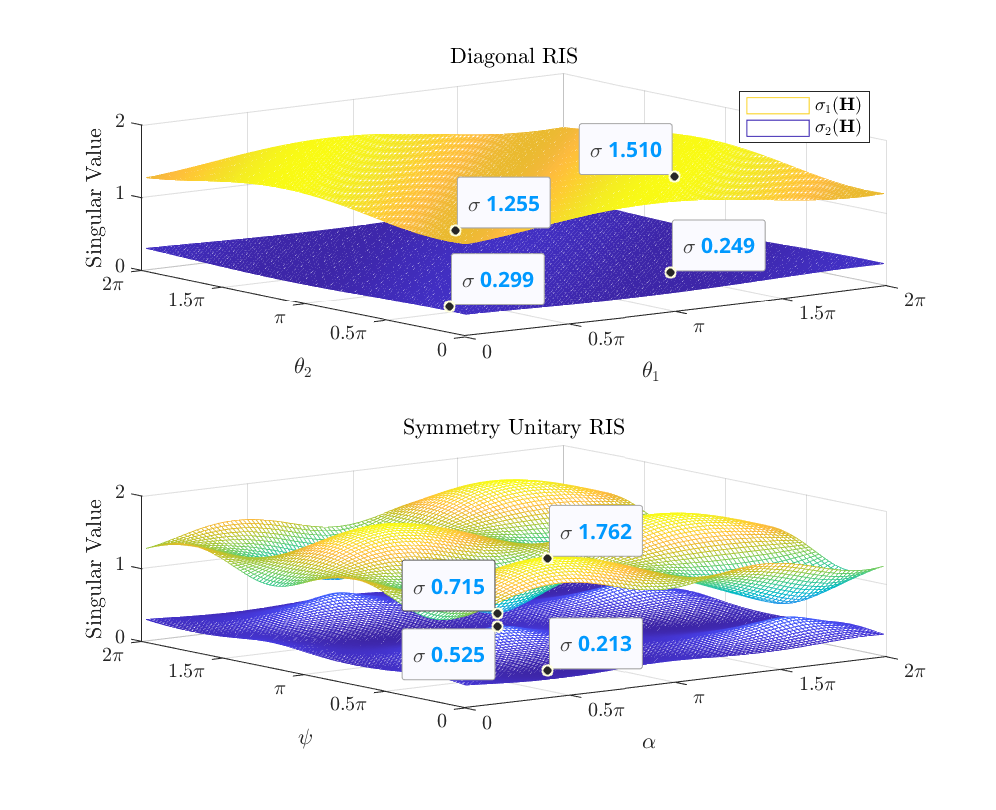
\includegraphics[width=\columnwidth]{assets/simulation/pc_singular_toy.eps}
			\caption{$2 \times 2 \times 2$ channel singular value shaping by diagonal and symmetry unitary \gls{ris}. Direct link is absent.}
			\label{sm:pc_singular_toy}
		\end{figure}
		Fig.~\ref{sm:pc_singular_toy} shows the channel singular values achieved by an exhaustive grid search over $(\theta_1, \theta_2)$ for diagonal \gls{ris} and $(\alpha, \psi)$ for symmetric unitary \gls{ris}.
		It is observed that both singular values can be manipulated up to $9\%$ using diagonal \gls{ris} and $42\%$ using symmetric \gls{bd}-\gls{ris}, despite both architectures have the same number of scattering elements and design parameters.
		A larger performance gap is expected when asymmetric \gls{bd}-\gls{ris} is available.
		This example shows \gls{bd}-\gls{ris} can provide a wider dynamic range of channel singular values and motivates further studies on channel shaping.
	\end{subsection}

	\begin{subsection}{Pareto Frontier Characterization}
		We then characterize the Pareto frontier of channel singular values by maximizing their weighted sum
		\begin{maxi!}
			{\scriptstyle{\mathbf{\Theta}}}{\sum_n \rho_n \sigma_n(\mathbf{H})}{\label{op:pareto}}{\label{ob:pareto}}
			\addConstraint{\mathbf{\Theta}_g^\mathsf{H} \mathbf{\Theta}_g=\mathbf{I},}{\quad \forall g,}{\label{co:pareto_unitary}}
		\end{maxi!}
		where $n \in \{1,\ldots,\min(N_\mathrm{T}, N_\mathrm{R})\}$ and $\rho_n$ is the weight of the $n$-th singular value that can be positive, zero, or negative.
		Varying $\{\rho_n\}$ unveils the entire achievable singular value region.
		Thus, the Pareto frontier problem~\eqref{op:pareto} generalizes most relevant metrics and provides a powerful shaping framework.
		The objective \eqref{ob:pareto} is smooth in $\mathbf{\Theta}$ and the feasible domain \eqref{co:pareto_unitary} for group $g$ corresponds to the Stiefel manifold.
		Next, we zoom out to general smooth maximization problems of asymmetric \gls{bd}-\gls{ris}.

		Inspired by \cite{Abrudan2008,Abrudan2009}, we propose a block-wise \gls{rcg} algorithm along the geodesics on the Lie group of unitary matrices $\mathbb{U}^{L \times L}$.
		It leverages the fact that unitary matrices are closed under multiplication.
		At iteration $r$, the gradient is computed in the Euclidean space and translated to the Riemannian manifold \cite{Absil2009}
		\begin{gather}
			\nabla_{\mathrm{E},g}^{(r)} = \frac{\partial f(\mathbf{\Theta}_g^{(r)})}{\partial \mathbf{\Theta}_g^*},\label{eq:gradient_euclidean}\\
			\nabla_{\mathrm{R},g}^{(r)} = \nabla_{\mathrm{E},g}^{(r)} {\mathbf{\Theta}_g^{(r)}}^\mathsf{H} - \mathbf{\Theta}_g^{(r)} {\nabla_{\mathrm{E},g}^{(r)}}^\mathsf{H}.\label{eq:gradient_riemannian}
		\end{gather}
		The Polak-Ribierre parameter \cite{Polak1969} is approximated as \cite{Abrudan2009}
		\begin{equation}
			\gamma_g^{(r)} = \frac{\mathrm{tr}\bigl((\nabla_{\mathrm{R},g}^{(r)} - \nabla_{\mathrm{R},g}^{(r-1)}) {\nabla_{\mathrm{R},g}^{(r)}}^\mathsf{H}\bigr)}{\mathrm{tr}\bigl(\nabla_{\mathrm{R},g}^{(r-1)} {\nabla_{\mathrm{R},g}^{(r-1)}}^\mathsf{H}\bigr)},
			\label{eq:parameter_cg}
		\end{equation}
		and the conjugate direction is
		\begin{equation}
			\mathbf{D}_g^{(r)} = \nabla_{\mathrm{R},g}^{(r)} + \gamma_g^{(r)} \mathbf{D}_g^{(r-1)}.
			\label{eq:direction_cg}
		\end{equation}
		In the Stiefel manifold, the geodesic emanating from $\mathbf{\Theta}_g^{(r)}$ with velocity $\mathbf{D}_g^{(r)}$ and step size $\mu$ is described compactly by the exponential map \cite{Edelman1998}
		\begin{equation}
			\mathbf{G}_g^{(r)}(\mu) = \exp(\mu \mathbf{D}_g^{(r)}) \mathbf{\Theta}_g^{(r)}.
			\label{eq:geodesic}
		\end{equation}
		An appropriate $\mu^\star$ can be obtained by the Armijo rule \cite{Armijo1966}.\footnote{To double the step size, one only need to square the rotation matrix instead of recomputing the matrix exponential, i.e., $\exp(2 \mu \mathbf{D}_g^{(r)}) = \exp^2(\mu \mathbf{D}_g^{(r)})$.}
		Finally, the scattering matrix is updated along the geodesic as
		\begin{equation}
			\mathbf{\Theta}_g^{(r+1)} = \mathbf{G}_g^{(r)}(\mu^\star).
			\label{eq:update_geodesic}
		\end{equation}
		Algorithm~\ref{ag:rcg} summarizes the proposed block-wise geodesic \gls{rcg} method for smooth maximization problems of asymmetric \gls{bd}-\gls{ris}.
		Convergence to stationary points is guaranteed as updating each block iteratively does not reduce the objective function.

		\begin{remark}
			Compared with universal manifold optimization \cite{Absil2009,Pan2022d}, Algorithm~\ref{ag:rcg} inherits a trifold benefit from \cite{Abrudan2008,Abrudan2009}:
			\begin{enumerate}
				\item No retraction thanks to rotational update \eqref{eq:geodesic}, \eqref{eq:update_geodesic};
				\item Lower computational complexity per iteration;
				\item Faster convergence thanks to proper parameter space.
			\end{enumerate}
		\end{remark}

		\setalgorithmcaptionfont{\small}
		\begin{algorithm}[!t]
			\small
			\caption{Block-wise geodesic \gls{rcg} for asymmetric \gls{bd}-\gls{ris}}
			\label{ag:rcg}
			\begin{algorithmic}[1]
				\Require $f(\mathbf{\Theta})$, $G$
				\Ensure $\mathbf{\Theta}^\star$
				\Initialize {$r \gets 0$, $\mathbf{\Theta}^{(0)}$}
				\Repeat
					\For {$g \gets 1$ to $G$}
						\State $\nabla_{\mathrm{E},g}^{(r)} \gets$ \eqref{eq:gradient_euclidean} \label{ln:gradient_euclidean}
						\State $\nabla_{\mathrm{R},g}^{(r)} \gets$ \eqref{eq:gradient_riemannian}
						\State $\gamma_g^{(r)} \gets$ \eqref{eq:parameter_cg}
						\State $\mathbf{D}_g^{(r)} \gets$ \eqref{eq:direction_cg}
						\If {$\Re\bigl\{\mathrm{tr}({\mathbf{D}_g^{(r)}}^\mathsf{H} \nabla_{\mathrm{R},g}^{(r)})\bigr\} < 0$} \Comment{not an ascent direction}
							\State $\mathbf{D}_g^{(r)} \gets \nabla_{\mathrm{R},g}^{(r)}$
						\EndIf
						\State $\mu \gets 1$
						\State $\mathbf{G}_g^{(r)}(\mu) \gets$ \eqref{eq:geodesic}
						\While {$f\bigl(\mathbf{G}_g^{(r)}(2\mu)\bigr) - f(\mathbf{\Theta}_g^{(r)}) \ge \mu \cdot \mathrm{tr}(\mathbf{D}_g^{(r)} {\mathbf{D}_g^{(r)}}^\mathsf{H}) / 2$}
							\State $\mu \gets 2 \mu$
						\EndWhile
						\While {$f\bigl(\mathbf{G}_g^{(r)}(\mu)\bigr) - f(\mathbf{\Theta}_g^{(r)}) < \mu / 2 \cdot \mathrm{tr}(\mathbf{D}_g^{(r)} {\mathbf{D}_g^{(r)}}^\mathsf{H}) / 2$}
							\State $\mu \gets \mu / 2$
						\EndWhile
						\State $\mathbf{\Theta}_g^{(r+1)} \gets$ \eqref{eq:update_geodesic}
					\EndFor
					\State $r \gets r+1$
				\Until $\lvert f(\mathbf{\Theta}^{(r)}) - f(\mathbf{\Theta}^{(r-1)}) \rvert / f(\mathbf{\Theta}^{(r-1)}) \le \epsilon$
			\end{algorithmic}
		\end{algorithm}

		% The Pareto singular value problem \eqref{op:pareto} can thus be solved by Algorithm~\ref{ag:rcg}.
		\begin{lemma}
			The Euclidean gradient of \eqref{ob:pareto} w.r.t. \gls{bd}-\gls{ris} group $g$ is
			\begin{equation}
				\frac{\partial \sum_n \rho_n \sigma_n(\mathbf{H})}{\partial \mathbf{\Theta}_g^*} = \mathbf{H}_{\mathrm{B},g}^\mathsf{H} \mathbf{U} \mathrm{diag}(\rho_1,\ldots,\rho_N) \mathbf{V}^\mathsf{H} \mathbf{H}_{\mathrm{F},g}^\mathsf{H},
				\label{eq:pareto_gradient}
			\end{equation}
			where $\mathbf{U} \in \mathbb{C}^{N_\mathrm{R} \times N}$ and $\mathbf{V} \in \mathbb{C}^{N_\mathrm{T} \times N}$ are the left and right compact singular matrices of $\mathbf{H}$, respectively.
		\end{lemma}
		\begin{proof}
			Let $\mathbf{H} = \sum_n \mathbf{u}_n \sigma_n \mathbf{v}_n^\mathsf{H}$ be the compact \gls{svd} of the equivalent channel.
			Since the singular vectors are orthonormal, the $n$-th singular value can be expressed as
			\begin{equation}
				\sigma_n = \mathbf{u}_n^\mathsf{H} \mathbf{H} \mathbf{v}_n = \mathbf{u}_n^\mathsf{T} \mathbf{H}^* \mathbf{v}_n^*,
			\end{equation}
			whose differential w.r.t. $\mathbf{\Theta}_g^*$ is
			\begin{align*}
				\partial \sigma_n
				& = \partial \mathbf{u}_n^\mathsf{T} \underbrace{\mathbf{H}^* \mathbf{v}_n^*}_{\sum_m \mathbf{u}_m^* \sigma_m \mathbf{v}_m^\mathsf{T} \mathbf{v}_n} + \mathbf{u}_n^\mathsf{T} \cdot \partial \mathbf{H}^* \cdot \mathbf{v}_n^* + \underbrace{\mathbf{u}_n^\mathsf{T} \mathbf{H}^*}_{\mathbf{u}_n^\mathsf{T} \sum_m \mathbf{u}_m^* \sigma_m \mathbf{v}_m^\mathsf{T}} \partial \mathbf{v}_n^*\\
				& = \underbrace{\partial \mathbf{u}_n^\mathsf{T} \mathbf{u}_n^*}_{\partial 1 = 0} \cdot \sigma_n + \mathbf{u}_n^\mathsf{T} \cdot \partial \mathbf{H}^* \cdot \mathbf{v}_n^* + \sigma_n \cdot \underbrace{\mathbf{v}_n^\mathsf{T} \partial \mathbf{v}_n^*}_{\partial 1 = 0}\\
				& = \mathbf{u}_n^\mathsf{T} \mathbf{H}_{\mathrm{B},g}^\mathsf{H} \cdot \partial \mathbf{\Theta}_g^* \cdot \mathbf{H}_{\mathrm{F},g}^* \mathbf{v}_n^*\\
				& = \mathrm{tr}(\mathbf{H}_{\mathrm{F},g}^* \mathbf{v}_n^*\mathbf{u}_n^\mathsf{T} \mathbf{H}_{\mathrm{B},g}^\mathsf{H} \cdot \partial \mathbf{\Theta}_g^*).
			\end{align*}
			According to \cite{Hjorungnes2007}, the corresponding complex derivative is
			\begin{equation}
				\frac{\partial \sigma_n}{\partial \mathbf{\Theta}_g^*} = \mathbf{H}_{\mathrm{B},g}^\mathsf{H} \mathbf{u}_n \mathbf{v}_n^\mathsf{H} \mathbf{H}_{\mathrm{F},g}^\mathsf{H}.
				\label{eq:derivative_sv}
			\end{equation}
			Linear combination of \eqref{eq:derivative_sv} yields \eqref{eq:pareto_gradient}.
		\end{proof}

		%  The Euclidean gradient of \gls{bd}-\gls{ris} group $g$ is computed as
		% where $\mathbf{U} \in \mathbb{C}^{N_\mathrm{R} \times N}$ and $\mathbf{V} \in \mathbb{C}^{N_\mathrm{T} \times N}$ are the left and right compact singular matrices of $\mathbf{H}$, respectively.
		Algorithm~\ref{ag:rcg} can thus be invoked for the Pareto singular value problem \eqref{op:pareto}, where line \ref{ln:gradient_euclidean} uses explicit expression \eqref{eq:pareto_gradient}.
		% \eqref{eq:pareto_gradient} is used in line \ref{ln:gradient_euclidean}.
	\end{subsection}

	\begin{subsection}{Some Analytical Bounds}
		We then discuss some analytical bounds related to channel singular values.
		\begin{proposition}[rank-deficient channel]
			In point-to-point \gls{mimo}, \gls{bd}-\gls{ris} cannot achieve a higher \gls{dof} than diagonal \gls{ris}.
		\end{proposition}
		\begin{proof}
			The scattering matrix of \gls{bd}-\gls{ris} can be decomposed as\footnote{This is because (block) unitary matrices are closed under multiplication.}
			\begin{equation}
				\mathbf{\Theta} = \mathbf{L} \mathbf{\Theta}_\mathrm{D} \mathbf{R}^\mathsf{H},
			\end{equation}
			where $\mathbf{\Theta}_\mathrm{D} \in \mathbb{U}^{N_\mathrm{S} \times N_\mathrm{S}}$ corresponds to diagonal \gls{ris} and $\mathbf{L}, \mathbf{R} \in \mathbb{U}^{N_\mathrm{S} \times N_\mathrm{S}}$ are block diagonal matrices of $L \times L$ unitary blocks.
			Manipulating $\mathbf{L}$ and $\mathbf{R}$ rotates the linear spans of $\bar{\mathbf{H}}_\mathrm{B} \triangleq \mathbf{H}_\mathrm{B} \mathbf{L}$ and $\bar{\mathbf{H}}_\mathrm{F} \triangleq \mathbf{R}^\mathsf{H} \mathbf{H}_\mathrm{F}$ and maintains their rank.
			On the other hand, there exists a $\mathbf{\Theta}_\mathrm{D}$ such that
			\begin{equation*}
				\begin{split}
					\mathrm{rank}(\mathbf{H}_\mathrm{B} \mathbf{\Theta}_\mathrm{D} \mathbf{H}_\mathrm{F})
					& = \min \bigl( \mathrm{rank}(\mathbf{H}_\mathrm{B}), \mathrm{rank}(\mathbf{\Theta}_\mathrm{D}), \mathrm{rank}(\mathbf{H}_\mathrm{F}) \bigr) \\
					& = \min \bigl( \mathrm{rank}(\bar{\mathbf{H}}_\mathrm{B}), N_\mathrm{S}, \mathrm{rank}(\bar{\mathbf{H}}_\mathrm{F}) \bigr) \\
					& = \max_\mathbf{\Theta} \ \mathrm{rank}(\mathbf{H}_\mathrm{B} \mathbf{\Theta} \mathbf{H}_\mathrm{F})
				\end{split}
			\end{equation*}
			The same result holds if the direct link is present.
		\end{proof}

		\begin{proposition}[\gls{los} forward\footnote{A similar result holds for \gls{los} backward channel.} channel]
			If the forward channel is rank-1, then \gls{bd}-\gls{ris} can at most enlarge (resp. suppress) the $n$-th ($n \ge 2$) channel singular value to the $(n-1)$-th (resp. $n$-th) singular value of $\mathbf{T}$, that is,
			\begin{equation}
				\sigma_1(\mathbf{T}) \ge {\sigma_2(\mathbf{H})} \ge \sigma_2(\mathbf{T}) \ge \ldots \ge \sigma_{N-1}(\mathbf{T}) \ge {\sigma_N(\mathbf{H})} \ge \sigma_N(\mathbf{T}),
				\label{iq:sv_bound_los}
			\end{equation}
			where $\mathbf{T} \mathbf{T}^\mathsf{H} = \mathbf{H}_\mathrm{D} (\mathbf{I} - \mathbf{v}_\mathrm{F} \mathbf{v}_\mathrm{F}^\mathsf{H}) \mathbf{H}_\mathrm{D}$ and $\mathbf{v}_\mathrm{F}$ is the right compact singular vector of $\mathbf{H}_\mathrm{F}$.
			Note that $\sigma_1(\mathbf{H})$ is unbounded with a sufficiently large \gls{ris}.
		\end{proposition}
		\begin{proof}
			Let $\mathbf{H}_\mathrm{F} = \sigma_\mathrm{F} \mathbf{u}_\mathrm{F} \mathbf{v}_\mathrm{F}^\mathsf{H}$ be the compact \gls{svd} of the forward channel.
			The channel Gram matrix can be written as Hermitian-plus-rank-1:
			\begin{equation}
				\mathbf{G} \triangleq \mathbf{H} \mathbf{H}^\mathsf{H} = \mathbf{Y} + \mathbf{z} \mathbf{z}^\mathsf{H},
			\end{equation}
			where $\mathbf{Y} \triangleq \mathbf{H}_\mathrm{D}^\mathsf{H} (\mathbf{I} - \mathbf{v}_\mathrm{F} \mathbf{v}_\mathrm{F}^\mathsf{H}) \mathbf{H}_\mathrm{D}$ and $\mathbf{z} \triangleq \sigma_\mathrm{F} \mathbf{H}_\mathrm{B} \mathbf{\Theta} \mathbf{u}_\mathrm{F} + \mathbf{H}_\mathrm{D} \mathbf{v}_\mathrm{F}$.
			By the Cauchy interlacing formula \cite{Golub2013}, the $n$-th ($n \ge 2$) eigenvalues of $\mathbf{G}$ are bounded by
			\begin{equation}
				\lambda_1(\mathbf{Y}) \ge \lambda_2(\mathbf{G}) \ge \lambda_2(\mathbf{Y}) \ge \ldots \ge \lambda_{N-1}(\mathbf{Y}) \ge \lambda_N(\mathbf{G}) \ge \lambda_N(\mathbf{Y}).
				\label{iq:ev_bound_los}
			\end{equation}
			Since $\mathbf{Y} = \mathbf{T} \mathbf{T}^\mathsf{H}$ is positive semi-definite, the eigenvalues are non-negative and taking the square root of \eqref{iq:ev_bound_los} gives \eqref{iq:sv_bound_los}.
		\end{proof}
		It is worth notice that a similar conclusion holds for diagonal \gls{ris} \cite{Semmler2023}.
		We will later show that for a finite $N_\mathrm{S}$, using a larger group size can approach those bounds better.

		\begin{proposition}[fully-connected \gls{ris} without direct link]
			% If the \gls{bd}-\gls{ris} is fully-connected and the direct link is absent, then the singular value bounds on $\mathbf{H}$ are equivalent to the singular value bounds on $\mathbf{BF}$, where $\mathbf{B}$ and $\mathbf{F}$ are arbitrary matrices with the same singular values as $\mathbf{H}_\mathrm{B}$ and $\mathbf{H}_\mathrm{F}$, respectively,
			If the \gls{bd}-\gls{ris} is fully-connected and the direct link is absent, then
			\begin{equation}
				\mathrm{sv}(\mathbf{H}) = \mathrm{sv}(\mathbf{BF}),
			\end{equation}
			where $\mathbf{B}$ and $\mathbf{F}$ are arbitrary matrices with the same singular values as $\mathbf{H}_\mathrm{B}$ and $\mathbf{H}_\mathrm{F}$, respectively,
		\end{proposition}

		\begin{proof}
			Let $\mathbf{H}_\mathrm{B} = \mathbf{U}_\mathrm{B} \mathbf{\Sigma}_\mathrm{B} \mathbf{V}_\mathrm{B}^\mathsf{H}$ and $\mathbf{H}_\mathrm{F} = \mathbf{U}_\mathrm{F} \mathbf{\Sigma}_\mathrm{F} \mathbf{V}_\mathrm{F}^\mathsf{H}$ be the \gls{svd} of the backward and forward channels, respectively.
			The scattering matrix of fully-connected \gls{ris} can be decomposed as
			\begin{equation}
				\mathbf{\Theta} = \mathbf{V}_\mathrm{B} \mathbf{X} \mathbf{U}_\mathrm{F}^\mathsf{H},
				\label{eq:scattering_fc}
			\end{equation}
			where $\mathbf{X} \in \mathbb{U}^{N_\mathrm{S} \times N_\mathrm{S}}$ is a unitary matrix to be designed.
			The equivalent channel is thus a function of $\mathbf{X}$
			\begin{equation}
				\mathbf{H} = \mathbf{H}_\mathrm{B} \mathbf{\Theta} \mathbf{H}_\mathrm{F} = \mathbf{U}_\mathrm{B} \mathbf{\Sigma}_\mathrm{B} \mathbf{X} \mathbf{\Sigma}_\mathrm{F} \mathbf{V}_\mathrm{F}^\mathsf{H}.
				\label{eq:channel_equivalent_fc}
			\end{equation}
			Since $\mathrm{sv}(\mathbf{U} \mathbf{A} \mathbf{V}^\mathsf{H}) = \mathrm{sv}(\mathbf{A})$ for unitary $\mathbf{U}$ and $\mathbf{V}$, we have
			\begin{align*}
				\mathrm{sv}(\mathbf{H}) & = \mathrm{sv}(\mathbf{U}_\mathrm{B} \mathbf{\Sigma}_\mathrm{B} \mathbf{X} \mathbf{\Sigma}_\mathrm{F} \mathbf{V}_\mathrm{F}^\mathsf{H})\\
				& = \mathrm{sv}(\mathbf{\Sigma}_\mathrm{B} \mathbf{X} \mathbf{\Sigma}_\mathrm{F})\\
				& = \mathrm{sv}(\bar{\mathbf{U}}_\mathrm{B} \mathbf{\Sigma}_\mathrm{B} \mathbf{\bar{V}}_\mathrm{B}^\mathsf{H} \bar{\mathbf{U}}_\mathrm{F} \mathbf{\Sigma}_\mathrm{F} \mathbf{\bar{V}}_\mathrm{F}^\mathsf{H})\\
				& = \mathrm{sv}(\mathbf{BF}),
			\end{align*}
			where $\bar{\mathbf{U}}_{\mathrm{B}/\mathrm{F}}$ and $\bar{\mathbf{V}}_{\mathrm{B}/\mathrm{F}}$ are arbitrary unitary matrices.
		\end{proof}

		There exist many singular value bounds on the product of two matrices in terms of their own singular values.
		One comprehensive answer is \cite{Fulton2000}
		\begin{equation}
			\prod_{k \in {K}} \sigma_k(\mathbf{H}) \le \prod_{i \in {I}} \sigma_i(\mathbf{H}_\mathrm{B}) \prod_{j \in {J}} \sigma_j(\mathbf{H}_\mathrm{F}),
			\label{iq:sv_bound_fc}
		\end{equation}
		for all admissible triples $(I, J, K) \in T_r^n$ with $r < n$, where
		\begin{equation}
			\begin{gathered}
				% T_r^n \triangleq \Bigl\{(I, J, K) \in U_r^n \mid \text{for all } p < r \text{ and all } (F, G, H) \text{ in } T_p^r,\\
				% \sum_{f \in F} i_f + \sum_{g \in G} j_g \le \sum_{h \in H} k_h + p(p+1)/2 \Bigr\},
				T_r^n \triangleq \Bigl\{(I, J, K) \in U_r^n \mid \forall p < r, (F, G, H) \in T_p^r,\\
				\sum_{f \in F} i_f + \sum_{g \in G} j_g \le \sum_{h \in H} k_h + p(p+1)/2 \Bigr\},
			\end{gathered}
		\end{equation}
		\begin{equation}
			U_r^n \triangleq \Bigl\{(I, J, K) \mid \sum_{i \in I} i + \sum_{j \in J} j = \sum_{k \in K} k + r(r+1)/2\Bigr\}.
		\end{equation}
		It implies the following special cases:
		\begin{itemize}
			\item upper bound on the largest singular value
			\begin{equation}
				\sigma_1(\mathbf{H}) \le \sigma_1(\mathbf{H}_\mathrm{B}) \sigma_1(\mathbf{H}_\mathrm{F});
			\end{equation}
			\item lower bound on the smallest singular value
			\begin{equation}
				\sigma_N(\mathbf{H}) \ge \sigma_N(\mathbf{H}_\mathrm{B}) \sigma_N(\mathbf{H}_\mathrm{F});
			\end{equation}
			\item upper bound on the product of first $k$ singular values
			\begin{equation}
				\prod_{n=1}^k \sigma_n(\mathbf{H}) \le \prod_{n=1}^k \sigma_n(\mathbf{H}_\mathrm{B}) \prod_{n=1}^k \sigma_n(\mathbf{H}_\mathrm{F});
			\end{equation}
			\item lower bound on the product of last $k$ singular values
			\begin{equation}
				\prod_{n=N}^{N-k+1} \sigma_n(\mathbf{H}) \ge \prod_{n=N}^{N-k+1} \sigma_n(\mathbf{H}_\mathrm{B}) \prod_{n=N}^{N-k+1} \sigma_n(\mathbf{H}_\mathrm{F});
			\end{equation}
			\item upper bound on the sum of first $k$ singular values to the power of $p > 0$
			\begin{equation}
				\sum_{n=1}^k \sigma_n^p(\mathbf{H}) \le \sum_{n=1}^k \sigma_n^p(\mathbf{H}_\mathrm{B}) \sigma_n^p(\mathbf{H}_\mathrm{F});
				\label{iq:sv_bound_fc_power}
			\end{equation}
			when $k = N$ and $p = 2$, it suggests the channel power is upper bounded by the sum of (sorted) element-wise power product of backward and forward subchannel.
		\end{itemize}

		\begin{remark}
			Interestingly, \eqref{iq:sv_bound_fc}--\eqref{iq:sv_bound_fc_power} are simultaneously tight when $\mathbf{\Theta} = \mathbf{V}_\mathrm{B} \mathbf{U}_\mathrm{F}^\mathsf{H}$.
			From \eqref{eq:scattering_fc} and \eqref{eq:channel_equivalent_fc}, we conclude the off-diagonal entries can enhance the capabilities of
			\begin{itemize}
				\item subspace alignment: $\mathbf{V}_\mathrm{B}$ and $\mathbf{U}_\mathrm{F}^\mathsf{H}$ in \eqref{eq:scattering_fc} fully align the subspaces of $\mathbf{H}_\mathrm{B}$ and $\mathbf{H}_\mathrm{F}$ by rotation;
				\item subchannel rearrangement: $\mathbf{X} = \mathbf{I}$ in \eqref{eq:channel_equivalent_fc} pairs the subchannels of $\mathbf{H}_\mathrm{B}$ and $\mathbf{H}_\mathrm{F}$ from strongest to weakest, which is optimal by rearrangement inequality.
			\end{itemize}
		\end{remark}

		Tight bounds are generally unavailable when \gls{mimo} direct link is present.
		This is because the \gls{ris} needs to balance the backward-forward (multiplicative) and direct-indirect (additive) subspace alignments.

		% \begin{figure}[!t]
		% 	\centering
		% 	\resizebox{0.65\columnwidth}{!}{
		% 		% This file was created by matlab2tikz.
%
%The latest updates can be retrieved from
%  http://www.mathworks.com/matlabcentral/fileexchange/22022-matlab2tikz-matlab2tikz
%where you can also make suggestions and rate matlab2tikz.
%
\definecolor{mycolor1}{rgb}{0.00000,0.44706,0.74118}%
\definecolor{mycolor2}{rgb}{0.85098,0.32549,0.09804}%
\definecolor{mycolor3}{rgb}{0.92941,0.69412,0.12549}%
\definecolor{mycolor4}{rgb}{0.49412,0.18431,0.55686}%
%
\begin{tikzpicture}

\begin{axis}[%
width=7.607cm,
height=6cm,
at={(0cm,0cm)},
scale only axis,
xmin=1.34996047912836,
xmax=3.72920240719628,
xlabel style={font=\color{white!15!black}},
xlabel={$\sigma_1$},
ymin=0.450747982664133,
ymax=2.80326064739205,
ylabel style={font=\color{white!15!black}},
ylabel={$\sigma_2$},
axis background/.style={fill=white},
xmajorgrids,
ymajorgrids,
legend style={at={(0.03,0.97)}, anchor=north west, legend cell align=left, align=left, draw=white!15!black},
every axis plot/.append style={line width=1.5pt}
]
\addplot[only marks, mark=triangle, mark options={}, mark size=2.3570pt, draw=black] table[row sep=crcr]{%
x	y\\
2.51354714236168	1.61586457213499\\
};
\addlegendentry{Direct}

\addplot [color=mycolor1, line width=2.0pt, mark=o, mark options={solid, mycolor1}]
  table[row sep=crcr]{%
1.61525947824021	1.51459941856087\\
1.61162946205727	1.49053812171925\\
1.62420465229831	1.37863429557545\\
1.65114733825308	1.26425569146059\\
1.69667404672018	1.16027147963777\\
1.79421133211752	1.02541660486879\\
1.93044773324239	0.902791601073093\\
2.06672961694553	0.817726556860225\\
2.17231094965278	0.774788170064984\\
2.30807839739658	0.744260885800279\\
2.47215488365949	0.727616873762207\\
};
\addlegendentry{$L = 1$}

\addplot [color=mycolor1, line width=2.0pt, mark=o, mark options={solid, mycolor1}, forget plot]
  table[row sep=crcr]{%
3.49185748027826	1.64721768664974\\
3.48506091132238	1.77113797636879\\
3.45882993148692	1.91650271116742\\
3.42264475913889	2.024316737542\\
3.354802290815	2.14756005128536\\
3.26698440553752	2.25390696995676\\
3.12914252593228	2.36621944248154\\
2.96430359319538	2.45475430666875\\
2.82595604339356	2.50137889225305\\
2.70561678332998	2.52245472965196\\
2.57907438393914	2.53116247419377\\
};
\addplot [color=mycolor2, dashed, line width=2.0pt, mark=+, mark options={solid, mycolor2}]
  table[row sep=crcr]{%
1.40572274282353	0.833358580446906\\
1.40291035344046	0.835920243006962\\
1.41044605905353	0.789966495453235\\
1.42532696219446	0.73927283635367\\
1.44902218081476	0.688578488170487\\
1.47828783930563	0.646413028752746\\
1.5156945348231	0.609413811311541\\
1.56095517475343	0.579109754372257\\
1.61007973294681	0.557538570811199\\
1.66271384037471	0.543676111867642\\
1.73417956504608	0.535496423730962\\
};
\addlegendentry{$L = 4$}

\addplot [color=mycolor2, dashed, line width=2.0pt, mark=+, mark options={solid, mycolor2}, forget plot]
  table[row sep=crcr]{%
3.68680616891169	2.31821034025669\\
3.68317716822127	2.39123511055662\\
3.67137066986446	2.45780285889309\\
3.65055479462623	2.52014590731068\\
3.6207921798012	2.5754081984725\\
3.5823181287399	2.62242492431761\\
3.53453672162676	2.66148724301662\\
3.47671803582177	2.69260139408801\\
3.41016630407252	2.71481046617056\\
3.33740136887	2.72768978052674\\
3.25909154187359	2.73182541427529\\
};
\addplot [color=mycolor3, dotted, line width=2.0pt, mark=square, mark options={solid, mycolor3}]
  table[row sep=crcr]{%
1.36454390992117	0.522251024232549\\
1.36449269131343	0.520129028903553\\
1.36544008284048	0.513824299237295\\
1.36738470679607	0.506362803641993\\
1.37044427255301	0.498876436819705\\
1.37515653692233	0.491416548866151\\
1.38069173991606	0.485486192445408\\
1.38641439144574	0.481298989744786\\
1.39350000471587	0.477787506259376\\
1.40197140927844	0.475197504207302\\
1.41168101053273	0.473589959917568\\
};
\addlegendentry{$L = 16$}

\addplot [color=mycolor3, dotted, line width=2.0pt, mark=square, mark options={solid, mycolor3}, forget plot]
  table[row sep=crcr]{%
3.71790799674737	2.66067885234264\\
3.71670169735444	2.68783623579614\\
3.71298904815406	2.70884198471926\\
3.70664674560816	2.72784984273427\\
3.69756142294611	2.74471184235163\\
3.68563623395784	2.75927993400713\\
3.67082796091405	2.77139102607105\\
3.65317890133333	2.78089376068831\\
3.63282831100592	2.78768064381891\\
3.61011583827057	2.79169457999857\\
3.58554850587157	2.79299541072653\\
};
\addplot [color=mycolor4, dashdotted, line width=2.0pt, mark=x, mark options={solid, mycolor4}]
  table[row sep=crcr]{%
1.34997031292588	0.464456322987329\\
1.34996047912836	0.464081450539269\\
1.35024079235631	0.462198587419813\\
1.35082209543419	0.459854115929761\\
1.35150776793345	0.45802550621846\\
1.35245596411905	0.456326412628538\\
1.35367888693481	0.454768407644107\\
1.3552991202949	0.453361512883599\\
1.35699694368241	0.452307959483886\\
1.35936091126519	0.451315630086337\\
1.36169477436734	0.450747982664133\\
};
\addlegendentry{$L = 64$}

\addplot [color=mycolor4, dashdotted, line width=2.0pt, mark=x, mark options={solid, mycolor4}, forget plot]
  table[row sep=crcr]{%
3.72920240719628	2.75328271480216\\
3.7287324987132	2.76219173164532\\
3.72729206646844	2.77033844061315\\
3.72481864043024	2.77775023071477\\
3.72126462973904	2.78434652870556\\
3.71660554708149	2.79003899762197\\
3.71081760804236	2.79477313756991\\
3.70392892473349	2.79848168263893\\
3.69595709994936	2.80114004860393\\
3.68692548022436	2.80273469890976\\
3.6769406316688	2.80326064739205\\
};
\end{axis}
\end{tikzpicture}%
		% 	}
		% 	\caption{Singular value Pareto frontier. $(N^\mathrm{T}, N^\mathrm{S}, N^\mathrm{R}) = (4, 64, 2)$, $(\Lambda^\mathrm{D}, \Lambda^\mathrm{F}, \Lambda^\mathrm{B}) = (0, -17.5, -17.5) \unit{dB}$.}
		% 	\label{sm:pc_singular_pareto}
		% \end{figure}

		% \begin{figure}[!t]
		% 	\centering
		% 	\resizebox{0.65\columnwidth}{!}{
		% 		% This file was created by matlab2tikz.
%
%The latest updates can be retrieved from
%  http://www.mathworks.com/matlabcentral/fileexchange/22022-matlab2tikz-matlab2tikz
%where you can also make suggestions and rate matlab2tikz.
%
\definecolor{mycolor1}{rgb}{0.58039,0.76863,0.96078}%
\definecolor{mycolor2}{rgb}{0.25882,0.37647,0.66667}%
\definecolor{mycolor3}{rgb}{0.94902,0.38039,0.38039}%
\definecolor{mycolor4}{rgb}{0.91765,0.03529,0.03529}%
\definecolor{mycolor5}{rgb}{0.46667,0.67451,0.18824}%
%
\begin{tikzpicture}

\begin{axis}[%
width=9.509cm,
height=7.5cm,
at={(0cm,0cm)},
scale only axis,
bar shift auto,
xmin=0,
xmax=5,
xtick={1,2,3,4},
xticklabels={{$\sigma_1$},{$\sigma_2$},{$\sigma_3$},{$\sigma_4$}},
ymin=0,
ymax=4.5,
ylabel style={font=\color{white!15!black}},
ylabel={Amplitude},
axis background/.style={fill=white},
xmajorgrids,
ymajorgrids,
legend style={legend cell align=left, align=left, draw=white!15!black},
legend columns=5,
transpose legend,
legend style={/tikz/column 2/.style={column sep=5pt}}
]
\addplot[ybar, bar width=0.123, fill=black, draw=black, area legend] table[row sep=crcr] {%
1	3.11578483462081\\
2	2.33621539044729\\
3	1.33501504737837\\
4	0.346232804852115\\
};
\addplot[forget plot, color=white!15!black] table[row sep=crcr] {%
0	0\\
5	0\\
};
\addlegendentry{Direct}

\addplot[ybar, bar width=0.123, fill=mycolor1, draw=black, area legend] table[row sep=crcr] {%
1	2.74905207049567\\
2	1.83843449000086\\
3	0.952844790933556\\
4	0.022527302733258\\
};
\addplot[forget plot, color=white!15!black] table[row sep=crcr] {%
0	0\\
5	0\\
};
\addlegendentry{Min, $L = 1$}

\addplot[ybar, bar width=0.123, fill=mycolor2, draw=black, area legend] table[row sep=crcr] {%
1	2.71936092735902\\
2	1.81605826060481\\
3	0.906339746943746\\
4	0.00914697809349159\\
};
\addplot[forget plot, color=white!15!black] table[row sep=crcr] {%
0	0\\
5	0\\
};
\addlegendentry{Min, $L = 32$}

\addplot[ybar, bar width=0.123, fill=mycolor3, draw=black, area legend] table[row sep=crcr] {%
1	3.8960081771894\\
2	2.67136418131802\\
3	1.64221742934803\\
4	0.603919247269453\\
};
\addplot[forget plot, color=white!15!black] table[row sep=crcr] {%
0	0\\
5	0\\
};
\addlegendentry{Max, $L = 1$}

\addplot[ybar, bar width=0.123, fill=mycolor4, draw=black, area legend] table[row sep=crcr] {%
1	4.03127940593837\\
2	2.67500105747776\\
3	1.67178857361767\\
4	0.628233917896107\\
};
\addplot[forget plot, color=white!15!black] table[row sep=crcr] {%
0	0\\
5	0\\
};
\addlegendentry{Max, $L = 32$}

\addplot [color=mycolor5, line width=2.0pt]
  table[row sep=crcr]{%
0	2.68074858002325\\
5	2.68074858002325\\
};
\addlegendentry{$\sigma_1(\mathbf{T})$}

\addplot [color=mycolor5, dashed, line width=2.0pt]
  table[row sep=crcr]{%
0	1.7029380545254\\
5	1.7029380545254\\
};
\addlegendentry{$\sigma_2(\mathbf{T})$}

\addplot [color=mycolor5, dotted, line width=2.0pt]
  table[row sep=crcr]{%
0	0.745179150575099\\
5	0.745179150575099\\
};
\addlegendentry{$\sigma_3(\mathbf{T})$}

\addplot [color=mycolor5, dashdotted, line width=2.0pt]
  table[row sep=crcr]{%
0	1.47492426026826e-08\\
5	1.47492426026826e-08\\
};
\addlegendentry{$\sigma_4(\mathbf{T})$}

\end{axis}

\begin{axis}[%
width=12.27cm,
height=9.202cm,
at={(-1.595cm,-1.012cm)},
scale only axis,
xmin=0,
xmax=1,
ymin=0,
ymax=1,
axis line style={draw=none},
ticks=none,
axis x line*=bottom,
axis y line*=left,
legend columns=5,
transpose legend,
legend style={/tikz/column 2/.style={column sep=5pt}}
]
\end{axis}
\end{tikzpicture}%
		% 	}
		% 	\caption{Singular value bounds for rank-1 indirect channel. $(N^\mathrm{T}, N^\mathrm{S}, N^\mathrm{R}) = (4, 32, 4)$, $(\Lambda^\mathrm{D}, \Lambda^\mathrm{F}, \Lambda^\mathrm{B}) = (0, -17.5, -17.5) \unit{dB}$.}
		% 	\label{sm:pc_singular_bound}
		% \end{figure}

		% The Pareto frontier and evolving trend of channel singular values are shown in Fig.~\ref{sm:pc_singular_pareto} and \ref{sm:pc_singular_bound}.
		% Clearly, \gls{bd}-\gls{ris} with a larger group size can redistribute the channel singular values to a wider range.
	\end{subsection}

\end{section}

\begin{section}{Rate Maximization}
	The \gls{mimo} rate maximization problem is formulated w.r.t. joint active and passive beamforming
	\begin{maxi!}
		{\scriptstyle{\mathbf{W},\mathbf{\Theta}}}{R = \log \det \biggl(\mathbf{I} + \frac{\mathbf{W}^\mathsf{H}\mathbf{H}^\mathsf{H}\mathbf{H}\mathbf{W}}{\eta}\biggr)}{\label{op:rate}}{\label{ob:rate}}
		\addConstraint{\lVert \mathbf{W} \rVert _\mathrm{F}^2 \le P}{}{}
		\addConstraint{\mathbf{\Theta}_g^\mathsf{H} \mathbf{\Theta}_g=\mathbf{I}, \quad \forall g,}{}{}
	\end{maxi!}
	where $\mathbf{W}$ is the transmit precoder, $R$ is the achievable rate, $\eta$ is the noise power, and $P$ is the transmit power budget.
	Two methods are proposed below to solve problem \eqref{op:rate}.

	\begin{subsection}{Alternating Optimization}
		We first consider an \gls{ao} approach that updates $\mathbf{\Theta}$ and $\mathbf{W}$ iteratively.
		For a given $\mathbf{W}$, the passive beamforming subproblem is
		\begin{maxi!}
			% {\scriptstyle{\mathbf{\Theta}}}{\log \det \biggl(\mathbf{I} + \frac{(\mathbf{H}_\mathrm{D} + \mathbf{H}_\mathrm{B} \mathbf{\Theta} \mathbf{H}_\mathrm{F}) \mathbf{Q} (\mathbf{H}_\mathrm{D}^\mathsf{H} + \mathbf{H}_\mathrm{F}^\mathsf{H} \mathbf{\Theta}^\mathsf{H} \mathbf{H}_\mathrm{B}^\mathsf{H})}{\eta}\biggr)}{\label{op:rate_passive}}{\label{ob:rate_passive}}
			{\scriptstyle{\mathbf{\Theta}}}{\log \det \biggl(\mathbf{I} + \frac{\mathbf{H} \mathbf{Q} \mathbf{H}^\mathsf{H}}{\eta}\biggr)}{\label{op:rate_passive}}{\label{ob:rate_passive}}
			\addConstraint{\mathbf{\Theta}_g^\mathsf{H} \mathbf{\Theta}_g=\mathbf{I}, \quad \forall g,}{}{}
		\end{maxi!}
		where $\mathbf{Q} \triangleq \mathbf{W} \mathbf{W}^\mathsf{H}$ is the transmit covariance matrix.
		\begin{lemma}
			The Euclidean gradient of \eqref{ob:rate_passive} w.r.t. \gls{bd}-\gls{ris} block $g$ is
			\begin{equation}
				\frac{\partial R}{\partial \mathbf{\Theta}_g^*} = \frac{1}{\eta} \mathbf{H}_{\mathrm{B},g}^\mathsf{H} \biggl(\mathbf{I} + \frac{\mathbf{H}\mathbf{Q}\mathbf{H}^\mathsf{H}}{\eta}\biggr)^{-1} \mathbf{H} \mathbf{Q} \mathbf{H}_{\mathrm{F},g}^\mathsf{H}.
				\label{eq:rate_gradient}
			\end{equation}
		\end{lemma}

		\begin{proof}
			The differential of $R$ w.r.t. $\mathbf{\Theta}_g^*$ is \cite{Hjorungnes2007}
			\begin{align*}
				\partial R
				& = \frac{1}{\eta} \mathrm{tr} \biggl\{ \partial \mathbf{H}^* \cdot \mathbf{Q}^\mathsf{T} \mathbf{H}^\mathsf{T} \Bigl(\mathbf{I} + \frac{\mathbf{H}^* \mathbf{Q}^\mathsf{T} \mathbf{H}^\mathsf{T}}{\eta}\Bigr)^{-1} \biggr\}\\
				& = \frac{1}{\eta} \mathrm{tr} \biggl\{ \mathbf{H}_{\mathrm{B},g}^* \cdot \partial \mathbf{\Theta}_g^* \cdot \mathbf{H}_{\mathrm{F},g}^* \mathbf{Q}^\mathsf{T} \mathbf{H}^\mathsf{T} \Bigl(\mathbf{I} + \frac{\mathbf{H}^* \mathbf{Q}^\mathsf{T} \mathbf{H}^\mathsf{T}}{\eta}\Bigr)^{-1} \biggr\}\\
				& = \frac{1}{\eta} \mathrm{tr} \biggl\{ \mathbf{H}_{\mathrm{F},g}^* \mathbf{Q}^\mathsf{T} \mathbf{H}^\mathsf{T} \Bigl(\mathbf{I} + \frac{\mathbf{H}^* \mathbf{Q}^\mathsf{T} \mathbf{H}^\mathsf{T}}{\eta}\Bigr)^{-1} \mathbf{H}_{\mathrm{B},g}^* \cdot \partial \mathbf{\Theta}_g^* \biggr\},
			\end{align*}
			and the corresponding complex derivative is \eqref{eq:rate_gradient}.
		\end{proof}
		Problem \eqref{op:rate_passive} is then solved by Algorithm \ref{ag:rcg}, where line \ref{ln:gradient_euclidean} uses explicit expression \eqref{eq:rate_gradient}.
		For a given $\mathbf{\Theta}$, the optimal transmit precoder is given by eigenmode transmission \cite{Clerckx2013}
		\begin{equation}
			\mathbf{W}^\star = \mathbf{V} {\mathbf{S}^\star}^{1/2},
		\end{equation}
		where $\mathbf{V}$ is the right singular matrix of $\mathbf{H}$ and $\mathbf{S}^\star$ is the optimal power allocation matrix obtained by the water-filling algorithm.
	\end{subsection}

	\begin{subsection}{Low-Complexity Solution}

	\end{subsection}

	% \begin{figure}[!t]
	% 	\centering
	% 	\subfloat[\gls{ris} Elements, $N^\mathrm{T} = 8$\label{sm:pc_rate_sx}]{
	% 		\resizebox{0.48\columnwidth}{!}{
	% 			% This file was created by matlab2tikz.
%
%The latest updates can be retrieved from
%  http://www.mathworks.com/matlabcentral/fileexchange/22022-matlab2tikz-matlab2tikz
%where you can also make suggestions and rate matlab2tikz.
%
\definecolor{mycolor1}{rgb}{0.00000,0.44706,0.74118}%
\definecolor{mycolor2}{rgb}{0.85098,0.32549,0.09804}%
%
\begin{tikzpicture}

\begin{axis}[%
width=7.607cm,
height=6cm,
at={(0cm,0cm)},
scale only axis,
xmin=-10,
xmax=30,
xlabel style={font=\color{white!15!black}},
xlabel={Direct SNR [dB]},
ymin=0,
ymax=60,
ylabel style={font=\color{white!15!black}},
ylabel={Achievable Rate [bit/s/Hz]},
axis background/.style={fill=white},
xmajorgrids,
ymajorgrids,
legend style={at={(0.03,0.97)}, anchor=north west, legend cell align=left, align=left, draw=white!15!black}
]
\addplot [color=black, line width=2.0pt]
  table[row sep=crcr]{%
-10	1.36546104868107\\
0	5.88537073819504\\
10	15.6479397698849\\
20	28.3545786367547\\
30	41.5803303056336\\
};
\addlegendentry{$N_s = 0$}

\addplot [color=mycolor1, line width=2.0pt, mark=o, mark options={solid, mycolor1}]
  table[row sep=crcr]{%
-10	1.58237983975058\\
0	6.50387837535644\\
10	16.8570947901563\\
20	29.7509492256546\\
30	42.9979138713491\\
};
\addlegendentry{$(N_s, L) = (32, 1)$}

\addplot [color=mycolor1, dashed, line width=2.0pt, mark=o, mark options={solid, mycolor1}]
  table[row sep=crcr]{%
-10	1.66761899571824\\
0	6.86015391678907\\
10	17.558641485772\\
20	30.5085404030891\\
30	43.7595094694537\\
};
\addlegendentry{$(N_s, L) = (32, 4)$}

\addplot [color=mycolor1, dotted, line width=2.0pt, mark=o, mark options={solid, mycolor1}]
  table[row sep=crcr]{%
-10	1.70198084326635\\
0	7.07761307084566\\
10	18.0075672651913\\
20	30.9873193827021\\
30	44.2430615141333\\
};
\addlegendentry{$(N_s, L) = (32, 32)$}

\addplot [color=mycolor2, line width=2.0pt, mark=+, mark options={solid, mycolor2}]
  table[row sep=crcr]{%
-10	3.12887098831763\\
0	10.3906425812424\\
10	22.8418905336598\\
20	36.0211679842767\\
30	49.2965127222328\\
};
\addlegendentry{$(N_s, L) = (256, 1)$}

\addplot [color=mycolor2, dashed, line width=2.0pt, mark=+, mark options={solid, mycolor2}]
  table[row sep=crcr]{%
-10	3.89754922195652\\
0	13.0217363041026\\
10	26.051145903396\\
20	39.2688611043277\\
30	52.5427674698922\\
};
\addlegendentry{$(N_s, L) = (256, 4)$}

\addplot [color=mycolor2, dotted, line width=2.0pt, mark=+, mark options={solid, mycolor2}]
  table[row sep=crcr]{%
-10	4.21684458588047\\
0	14.1060943448495\\
10	27.9675046836052\\
20	41.2102781687149\\
30	54.4927123740025\\
};
\addlegendentry{$(N_s, L) = (256, 256)$}

\end{axis}
\end{tikzpicture}%
	% 		}
	% 	}
	% 	\subfloat[Transmit Antenna, $N^\mathrm{S} = 256$\label{sm:pc_rate_tx}]{
	% 		\resizebox{0.48\columnwidth}{!}{
	% 			% This file was created by matlab2tikz.
%
%The latest updates can be retrieved from
%  http://www.mathworks.com/matlabcentral/fileexchange/22022-matlab2tikz-matlab2tikz
%where you can also make suggestions and rate matlab2tikz.
%
\definecolor{mycolor1}{rgb}{0.00000,0.44706,0.74118}%
\definecolor{mycolor2}{rgb}{0.85098,0.32549,0.09804}%
\definecolor{mycolor3}{rgb}{0.92941,0.69412,0.12549}%
%
\begin{tikzpicture}

\begin{axis}[%
width=9.509cm,
height=7.5cm,
at={(0cm,0cm)},
scale only axis,
xmin=-10,
xmax=30,
% xlabel style={font=\color{white!15!black}},
xlabel={Direct SNR [dB]},
ymin=0,
ymax=60,
% ylabel style={font=\color{white!15!black}},
ylabel={Achievable Rate [bit/s/Hz]},
axis background/.style={fill=white},
xmajorgrids,
ymajorgrids,
legend style={at={(0.03,0.97)}, anchor=north west, legend cell align=left, align=left, draw=white!15!black}
]
\addplot [color=mycolor1, line width=2.0pt, mark=o, mark options={solid, mycolor1}]
  table[row sep=crcr]{%
-10	1.82485438191362\\
0	4.7222906563119\\
10	7.99393509732638\\
20	11.3107371667968\\
30	14.6321519880831\\
};
\addlegendentry{$(N^\mathrm{T}, L) = (1, 1)$}

\addplot [color=mycolor1, dashed, line width=2.0pt, mark=o, mark options={solid, mycolor1}]
  table[row sep=crcr]{%
-10	2.24659926648999\\
0	5.26330445507328\\
10	8.55078517680736\\
20	11.8692222057207\\
30	15.1908007320325\\
};
\addlegendentry{$(N^\mathrm{T}, L) = (1, 256)$}

\addplot [color=mycolor2, line width=2.0pt, mark=+, mark options={solid, mycolor2}]
  table[row sep=crcr]{%
-10	2.49039510987196\\
0	8.06192104582032\\
10	17.6588170852107\\
20	32.7099587384036\\
30	45.9789160838128\\
};
\addlegendentry{$(N^\mathrm{T}, L) = (4, 1)$}

\addplot [color=mycolor2, dashed, line width=2.0pt, mark=+, mark options={solid, mycolor2}]
  table[row sep=crcr]{%
-10	3.77849180447307\\
0	13.3359194935281\\
10	26.0483499099173\\
20	39.2753832167713\\
30	52.5569826592083\\
};
\addlegendentry{$(N^\mathrm{T}, L) = (4, 256)$}

\addplot [color=mycolor3, line width=2.0pt, mark=square, mark options={solid, mycolor3}]
  table[row sep=crcr]{%
-10	3.8179809156775\\
0	12.9043718464691\\
10	25.5833268533688\\
20	38.8067308900334\\
30	52.0881220415066\\
};
\addlegendentry{$(N^\mathrm{T}, L) = (16, 1)$}

\addplot [color=mycolor3, dashed, line width=2.0pt, mark=square, mark options={solid, mycolor3}]
  table[row sep=crcr]{%
-10	5.83961863479039\\
0	16.7543020939844\\
10	29.7401886345762\\
20	42.9967723667009\\
30	56.2807797979848\\
};
\addlegendentry{$(N^\mathrm{T}, L) = (16, 256)$}

\end{axis}

\begin{axis}[%
width=12.27cm,
height=9.202cm,
at={(-1.595cm,-1.012cm)},
scale only axis,
xmin=0,
xmax=1,
ymin=0,
ymax=1,
axis line style={draw=none},
ticks=none,
axis x line*=bottom,
axis y line*=left
]
\end{axis}
\end{tikzpicture}%

	% 		}
	% 	}
	% 	\caption{Average achievable rate versus group size $L$. $N^\mathrm{R} = 4$, $(\Lambda^\mathrm{D}, \Lambda^\mathrm{F}, \Lambda^\mathrm{B}) = (65, 54, 46) \unit{dB}$.}
	% 	\label{sm:pc_rate}
	% \end{figure}

	% Fig.~\ref{sm:pc_rate_sx} illustrates how \gls{ris} configuration influences the \gls{mimo} \gls{pc} achievable rate.
	% To ensure a \qty{20}{bit/s/Hz} transmission, an \gls{snr} of \qty{13.5}{\dB} is required for a 8T4R system.
	% This value decreases to \qty{12.5}{\dB} (resp. \qty{8}{\dB}) when 32- (resp. 256-) element diagonal \gls{ris} is present.
	% If tetrads can be formed in \gls{bd}-\gls{ris}, the \gls{snr} can be reduced by another \qty{20}{\percent} (resp. \qty{44}{\percent}).
	% Further increase in $L$ yields a marginal gain and incurs $\mathcal{O}(L^2)$ connections.
	% We thus conclude dyadic or tetradic \gls{bd}-\gls{ris} usually strike a good balance between performance and complexity.


	\begin{subsection}{Channel Power Maximization}
		Consider a \gls{bd}-\gls{ris} with $N^\mathrm{S}$ elements, which is divided into $G$ groups of equal $L$ elements.
		\begin{maxi!}
			{\scriptstyle{\mathbf{\Theta}}}{\left\lVert \mathbf{H}^\mathrm{D} + \sum_g\nolimits \mathbf{H}_g^\mathrm{B} \mathbf{\Theta}_g \mathbf{H}_g^\mathrm{F} \right\rVert _\mathrm{F}^2}{\label{op:pc_power}}{}
			\addConstraint{\mathbf{\Theta}_g^\mathsf{H} \mathbf{\Theta}_g=\mathbf{I}, \quad \forall g \in \mathcal{G} \triangleq \{1,\ldots,G\}.}{}{}
		\end{maxi!}
		For \emph{symmetric} BD-RIS, the problem has been solved in
		\begin{itemize}
			\item Matteo's paper \cite{Nerini2023}: SISO and equivalent\footnote{Single-stream MIMO with given precoder and combiner.};
			\item Ignacio's paper \cite{Santamaria2023}: SISO and directless MISO/SIMO.
		\end{itemize}

		\begin{remark}
			% The difficulty of \eqref{op:pc_power} is that the \gls{ris} needs to balance the (additive) direct-indirect eigenspace alignment and the (multiplicative) forward-backward eigenspace alignment.
			The difficulty of \eqref{op:pc_power} is that the \gls{ris} needs to balance the additive (direct-indirect) and multiplicative (forward-backward) eigenspace alignment.
			% align the direct and indirect eigenspaces while preserving the
			Interestingly, it has the same form as the \emph{weighted orthogonal Procrustes problem} \cite{Gower2004}:
			\begin{mini!}
				{\scriptstyle{\mathbf{\Theta}}}{\lVert \mathbf{C} - \mathbf{A \Theta B} \rVert _\mathrm{F}^2}{\label{op:weighted_orthogonal_procrustes}}{}
				\addConstraint{\mathbf{\Theta}^\mathsf{H} \mathbf{\Theta}=\mathbf{I}.}{}{}
			\end{mini!}
			There exists no trivial solution to \eqref{op:weighted_orthogonal_procrustes}.
			One lossy transformation, by moving $\mathbf{\Theta}$ to one side \cite{Bell2003}, formulates a standard orthogonal Procrustes problem:
			\begin{mini!}
				{\scriptstyle{\mathbf{\Theta}}}{\lVert \mathbf{A}^\dagger \mathbf{C} - \mathbf{\Theta B} \rVert _\mathrm{F}^2}{\label{op:standard_orthogonal_procrustes}}{}
				\addConstraint{\mathbf{\Theta}^\mathsf{H} \mathbf{\Theta}=\mathbf{I}.}{}{}
			\end{mini!}
			\eqref{op:standard_orthogonal_procrustes} has a global optimal solution $\mathbf{\Theta}^\star = \mathbf{U} \mathbf{V}^\mathsf{H}$, where $\mathbf{U}$ and $\mathbf{V}$ are left and right singular matrix of $\mathbf{\mathbf{A}^\dagger \mathbf{C} \mathbf{B}^\mathsf{H}}$ \cite{Golub2013}.
			This low-complexity solution will be compared with the one proposed later.
		\end{remark}

		Inspired by \cite{Nie2017}, we propose an iterative algorithm to solve \eqref{op:pc_power}.
		The idea is to successively approximate the quadratic objective with a sequence of affine functions and solve the resulting subproblems in closed form.

		\begin{proposition}
			Start from any $\mathbf{\Theta}^{(0)}$, the sequence
			\begin{equation}
				\mathbf{\Theta}_g^{(r+1)} = \mathbf{U}_g^{(r)} \mathbf{V}_g^{(r)}, \quad \forall g
			\end{equation}
			converges to a stationary point of \eqref{op:pc_power}, where $\mathbf{U}_g^{(r)}$ and $\mathbf{V}_g^{(r)}$ are left and right singular matrix of
			\begin{equation}
				\begin{split}
					\mathbf{M}_g^{(r)}
					& = {\mathbf{H}_g^\mathrm{B}}^\mathsf{H} \mathbf{H}^\mathrm{D} {\mathbf{H}_g^\mathrm{F}}^\mathsf{H} + \sum_{g' < g} {\mathbf{H}_{g'}^\mathrm{B}}^\mathsf{H} \mathbf{H}_{g'}^\mathrm{B} \mathbf{\Theta}_{g'}^{(r+1)} \mathbf{H}_{g'}^\mathrm{F} {\mathbf{H}_{g'}^\mathrm{F}}^\mathsf{H} \\
					& \quad + \sum_{g' \ge g} {\mathbf{H}_{g'}^\mathrm{B}}^\mathsf{H} \mathbf{H}_{g'}^\mathrm{B} \mathbf{\Theta}_{g'}^{(r)} \mathbf{H}_{g'}^\mathrm{F} {\mathbf{H}_{g'}^\mathrm{F}}^\mathsf{H}.
				\end{split}
			\end{equation}
		\end{proposition}

		\begin{proof}
			To be added.
		\end{proof}

		\begin{figure}[!t]
			\centering
			\resizebox{0.65\columnwidth}{!}{
				% This file was created by matlab2tikz.
%
%The latest updates can be retrieved from
%  http://www.mathworks.com/matlabcentral/fileexchange/22022-matlab2tikz-matlab2tikz
%where you can also make suggestions and rate matlab2tikz.
%
\definecolor{mycolor1}{rgb}{0.85098,0.32549,0.09804}%
\definecolor{mycolor2}{rgb}{0.92941,0.69412,0.12549}%
\definecolor{mycolor3}{rgb}{0.49412,0.18431,0.55686}%
\definecolor{mycolor4}{rgb}{0.46667,0.67451,0.18824}%
%
\begin{tikzpicture}

\begin{axis}[%
width=7.607cm,
height=6cm,
at={(0cm,0cm)},
scale only axis,
xmin=0,
xmax=8,
xtick={0,1,2,3,4,5,6,7,8},
xticklabels={{$2^0$},{$2^1$},{$2^2$},{$2^3$},{$2^4$},{$2^5$},{$2^6$},{$2^7$},{$2^8$}},
xlabel style={font=\color{white!15!black}},
xlabel={RIS Group Size},
ymin=0,
ymax=7e-05,
ylabel style={font=\color{white!15!black}},
ylabel={Channel Power [W]},
axis background/.style={fill=white},
xmajorgrids,
ymajorgrids,
legend style={at={(0.03,0.97)}, anchor=north west, legend cell align=left, align=left, draw=white!15!black}
]
\addplot [color=black, line width=2.0pt]
  table[row sep=crcr]{%
0	9.99481299849178e-06\\
8	9.99481299849178e-06\\
};
\addlegendentry{$N_s = 0$}

\addplot [color=mycolor1, dashed, line width=2.0pt, mark=+, mark options={solid, mycolor1}]
  table[row sep=crcr]{%
0	1.02065060534792e-05\\
1	1.02857052718835e-05\\
2	1.03657178891351e-05\\
};
\addlegendentry{$N_s = 4$}

\addplot [color=mycolor2, dotted, line width=2.0pt, mark=square, mark options={solid, mycolor2}]
  table[row sep=crcr]{%
0	1.08240394393943e-05\\
1	1.11240963559512e-05\\
2	1.14708685265676e-05\\
3	1.16901587097421e-05\\
4	1.17920396956223e-05\\
};
\addlegendentry{$N_s = 16$}

\addplot [color=mycolor3, dashdotted, line width=2.0pt, mark=x, mark options={solid, mycolor3}]
  table[row sep=crcr]{%
0	1.38635087399098e-05\\
1	1.53706530394954e-05\\
2	1.70408162342293e-05\\
3	1.82388146554718e-05\\
4	1.88521652325586e-05\\
5	1.92013834134077e-05\\
6	1.93951032304193e-05\\
};
\addlegendentry{$N_s = 64$}

\addplot [color=mycolor4, line width=2.0pt, mark=triangle, mark options={solid, mycolor4}]
  table[row sep=crcr]{%
0	2.97266633680327e-05\\
1	3.79660436735737e-05\\
2	4.94606552637649e-05\\
3	5.8335214274755e-05\\
4	6.30806269398545e-05\\
5	6.56210846273517e-05\\
6	6.68339320816644e-05\\
7	6.76530541601078e-05\\
8	6.88056961056934e-05\\
};
\addlegendentry{$N_s = 256$}

\end{axis}

\begin{axis}[%
width=9.816cm,
height=7.362cm,
at={(-1.276cm,-0.81cm)},
scale only axis,
xmin=0,
xmax=1,
ymin=0,
ymax=1,
axis line style={draw=none},
ticks=none,
axis x line*=bottom,
axis y line*=left
]
\end{axis}
\end{tikzpicture}%
			}
			\caption{Average channel power versus \gls{ris} elements $N^\mathrm{S}$ and group size $L$. $(N^\mathrm{T}, N^\mathrm{R}) = (8, 4)$, $(\Lambda^\mathrm{D}, \Lambda^\mathrm{F}, \Lambda^\mathrm{B}) = (65, 54, 46) \unit{dB}$.}
			\label{sm:pc_power_sx}
		\end{figure}

		\begin{figure}[!t]
			\centering
			\subfloat[Without Direct Link\label{sm:pc_power_bond_nd}]{
				\resizebox{0.48\columnwidth}{!}{
					% This file was created by matlab2tikz.
%
%The latest updates can be retrieved from
%  http://www.mathworks.com/matlabcentral/fileexchange/22022-matlab2tikz-matlab2tikz
%where you can also make suggestions and rate matlab2tikz.
%
\definecolor{mycolor1}{rgb}{0.46667,0.67451,0.18824}%
\definecolor{mycolor2}{rgb}{0.92941,0.50588,0.59608}%
%
\begin{tikzpicture}

\begin{axis}[%
width=7.607cm,
height=6cm,
at={(0cm,0cm)},
scale only axis,
bar shift auto,
xmin=0,
xmax=6,
xtick={1,2,3,4,5},
xticklabels={{1},{4},{16},{64},{256}},
xlabel style={font=\color{white!15!black}},
xlabel={RIS Group Size},
ymin=0,
ymax=3.5e-05,
ylabel style={font=\color{white!15!black}},
ylabel={Channel Power [W]},
axis background/.style={fill=white},
xmajorgrids,
ymajorgrids,
legend style={at={(0.03,0.97)}, anchor=north west, legend cell align=left, align=left, draw=white!15!black}
]
\addplot[ybar, bar width=0.8, fill=mycolor1, draw=black, area legend] table[row sep=crcr] {%
1	7.67624350482862e-07\\
2	1.32530638063741e-06\\
3	3.06197930445936e-06\\
4	9.39519835024894e-06\\
5	3.02284526139409e-05\\
};
\addplot[forget plot, color=white!15!black] table[row sep=crcr] {%
0	0\\
6	0\\
};
\addlegendentry{Composite}

\addplot [color=black, line width=2.0pt]
  table[row sep=crcr]{%
-0.2	0\\
6.2	0\\
};
\addlegendentry{Direct}

\addplot [color=mycolor2, line width=2.0pt]
  table[row sep=crcr]{%
-0.2	3.04194803196479e-05\\
6.2	3.04194803196479e-05\\
};
\addlegendentry{Cascaded}

\end{axis}
\end{tikzpicture}%
				}
			}
			\subfloat[With Direct Link\label{sm:pc_power_bond_hd}]{
				\resizebox{0.48\columnwidth}{!}{
					% This file was created by matlab2tikz.
%
%The latest updates can be retrieved from
%  http://www.mathworks.com/matlabcentral/fileexchange/22022-matlab2tikz-matlab2tikz
%where you can also make suggestions and rate matlab2tikz.
%
\definecolor{mycolor1}{rgb}{0.46667,0.67451,0.18824}%
\definecolor{mycolor2}{rgb}{0.92941,0.50588,0.59608}%
%
\begin{tikzpicture}

\begin{axis}[%
width=7.607cm,
height=6cm,
at={(0cm,0cm)},
scale only axis,
bar shift auto,
xmin=0,
xmax=6,
xtick={1,2,3,4,5},
xticklabels={{1},{4},{16},{64},{256}},
xlabel style={font=\color{white!15!black}},
xlabel={RIS Group Size},
ymin=0,
ymax=7e-05,
ylabel style={font=\color{white!15!black}},
ylabel={Channel Power [W]},
axis background/.style={fill=white},
xmajorgrids,
ymajorgrids,
legend style={at={(0.03,0.97)}, anchor=north west, legend cell align=left, align=left, draw=white!15!black}
]
\addplot[ybar, bar width=0.8, fill=mycolor1, draw=black, area legend] table[row sep=crcr] {%
1	2.83336295997331e-05\\
2	4.76924466169225e-05\\
3	6.08890936283682e-05\\
4	6.46004645413477e-05\\
5	6.64188484186803e-05\\
};
\addplot[forget plot, color=white!15!black] table[row sep=crcr] {%
0	0\\
6	0\\
};
\addlegendentry{Composite}

\addplot [color=black, line width=2.0pt]
  table[row sep=crcr]{%
-0.2	9.51300474293446e-06\\
6.2	9.51300474293446e-06\\
};
\addlegendentry{Direct}

\addplot [color=mycolor2, line width=2.0pt]
  table[row sep=crcr]{%
-0.2	3.07152044114707e-05\\
6.2	3.07152044114707e-05\\
};
\addlegendentry{Cascaded}

\end{axis}
\end{tikzpicture}%
				}
			}
			\caption{Average channel power versus \gls{ris} group size $L$. $(N^\mathrm{T}, N^\mathrm{S}, N^\mathrm{R}) = (8, 256, 4)$, $(\Lambda^\mathrm{D}, \Lambda^\mathrm{F}, \Lambda^\mathrm{B}) = (65, 54, 46) \unit{dB}$.}
			\label{sm:pc_power_bond}
		\end{figure}
		% Fig.~\ref{sm:pc_power_sx} shows that, apart from numerous reflecting elements, a sufficiently large group size can help
		% Fig.~\ref{sm:pc_power_sx} shows that increasing the group size can improve the channel power especially for a large \gls{ris}.
		Fig.~\ref{sm:pc_power_sx} shows that, apart from adding reflecting elements $N^\mathrm{S}$, increasing the group size $L$ also improves the channel power.
		% The behavior is more obvious for a large \gls{ris}.
		This behavior is more pronounced for a large \gls{ris}.
		For example, the gain of pairwise connection is \qty{2.8}{\percent} for $N^\mathrm{S} = 16$ and \qty{28}{\percent} for $N^\mathrm{S} = 256$.
		% \gls{bd}-\gls{ris} provides a higher channel power than conventional \gls{ris}.
		% As $L$ increases from 1 to 2,
		It implies that the channel shaping capability of \gls{bd}-\gls{ris} scales with group size $L$.

		Fig.~\ref{sm:pc_power_bond_hd} and \ref{sm:pc_power_bond_nd} compare the average channel power without and with direct link.
		% where the cascaded channel power available to passive \gls{ris} is $\lVert \mathbf{H}^\mathrm{B} \rVert _\mathrm{F}^2 \lVert \mathbf{H}^\mathrm{F} \rVert _\mathrm{F}^2$.
		% where the cascaded channel power available to passive \gls{ris} is $\lVert \mathbf{H}^\mathrm{B} \rVert _\mathrm{F}^2 \lVert \mathbf{H}^\mathrm{F} \rVert _\mathrm{F}^2$.
		% ``Cascaded'' means the maximum power of the cascaded channel, i.e., $\lVert \mathbf{H}^\mathrm{B} \rVert _\mathrm{F}^2 \lVert \mathbf{H}^\mathrm{F} \rVert _\mathrm{F}^2$.
		% maximum power of the cascaded channel, i.e., $\lVert \mathbf{H}^\mathrm{B} \rVert _\mathrm{F}^2 \lVert \mathbf{H}^\mathrm{F} \rVert _\mathrm{F}^2$.
		% ? ``Cascaded'' means the \emph{power product} of the forward and backward channels.
		% ``Cascaded'' means the sum of element-wise product of first $N = \min(N^\mathrm{T}, N^\mathrm{S}, N^\mathrm{R})$ eigenvalues of the forward and backward channels.
		``Cascaded'' means the sum of element-wise product of first $N = \min(N^\mathrm{T}, N^\mathrm{S}, N^\mathrm{R})$ eigenvalues (i.e., element-wise power product) of the forward and backward channels.
		We observe that diagonal \gls{ris} wastes substantial cascaded power and struggles to align the direct-indirect eigenspace.
		When the direct link is absent, only \qty{2.6}{\percent} of available power is utilized by diagonal \gls{ris} while \qty{100}{\percent} power is recycled by fully-connected \gls{ris}.
		When the direct link is present, the proposed \gls{bd}-\gls{ris} design can balance the direct-indirect and forward-backward eigenspace alignment for an optimal channel boost.
		It is worth noting that, when $L$ is sufficiently large, the composite channel power surpasses the power sum of direct and cascaded channels, thanks to the constructive \emph{amplitude superposition} of direct and cascaded channels.
		This again emphasizes the advantage of in-group connection of \gls{bd}-\gls{ris}.
		% This is because the direct and indirect channels superpose
		% the proposed \gls{bd}-\gls{ris} design can also be applied to conventional \gls{ris} to improve the channel power.
		% When the direct link is present, a small $L$ cannot align the direct-indirect eigenspace.

		% neither effectively utilizes the cascaded channel power, nor effectively align the direct-indirect eigenspace.
		% We observe that conventional \gls{ris} neither effectively utilizes the cascaded channel power, nor effectively align the direct-indirect eigenspace.
		% For conventional \gls{ris},
		% align the direct-indirect eigenspace.
		% When the direct link is present, a small $L$ can neither align the direct-indirect eigenspace nor the forward-backward eigenspace.
		% For a relatively large $N^\mathrm{S}$, conventional \gls{ris} cannot
		% neither the direct-indirect nor the forward-backward eigenspace can be effectively aligned with a small $L$.

		% When the direct link is present, a small $L$ can neither preserve the
		% neither align the direct-indirect eigenspace nor the forward-backward eigenspace.

		% When the direct link is absent, a large $L$ can align the forward-backward eigenspace but cannot preserve the forward-backward power balance.
	\end{subsection}

\end{section}


\begin{section}{\glsentryshort{mimo}-\glsentryshort{ic}}
	\begin{subsection}{Leakage Interference Minimization}
		\begin{mini!}
			{\scriptstyle{\mathbf{\Theta}, \{\mathbf{G}_k\}, \{\mathbf{W}_k\}}}{\mathop{\sum\sum}_{j \neq k} \left\lVert \mathbf{G}_k (\mathbf{H}_{kj}^\mathrm{D} + \mathbf{H}_k^\mathrm{B} \mathbf{\Theta} \mathbf{H}_j^\mathrm{F}) \mathbf{W}_j \right\rVert _{\mathrm{F}}^2}{}{}
			\addConstraint{\mathbf{\Theta}_g^\mathsf{H} \mathbf{\Theta}_g=\mathbf{I}, \quad \forall g}{}{}
			\addConstraint{\mathbf{G}_k \mathbf{G}_k^\mathsf{H}=\mathbf{I}, \quad \mathbf{W}_k^\mathsf{H} \mathbf{W}_k=\mathbf{I}, \quad \forall k.}{}{}
		\end{mini!}
		The non-convex problem can be solved by \gls{bcd} method.
		For a given $\mathbf{\Theta}$, it reduces to conventional linear beamforming problem, for which an iterative algorithm alternating between the original and reciprocal networks is proposed in \cite{Gomadam2011,Clerckx2013}.
		At iteration $r$, the combiner at receiver $k$ is updated as
		\begin{equation}
			\mathbf{G}_k^{(r)} = {\mathbf{U}_{k,N}^{(r-1)}}^\mathsf{H},
		\end{equation}
		where $\mathbf{U}_{k,N}^{(r-1)}$ is the eigenvectors corresponding to $N$ smallest eigenvalues of interference covariance matrix $\mathbf{Q}_k^{(r-1)} = \sum_{j \ne k} \mathbf{H}_{kj} \mathbf{W}_j^{(r-1)} {\mathbf{W}_j^{(r-1)}}^\mathsf{H} \mathbf{H}_{kj}^\mathsf{H}$.
		The precoder at transmitter $j$ is updated as
		\begin{equation}
			\mathbf{W}_j^{(r)} = \bar{\mathbf{U}}_{j,N}^{(r)},
		\end{equation}
		where $\bar{\mathbf{U}}_{j,N}^{(r)}$ corresponds to interference covariance matrix $\bar{\mathbf{Q}}_j^{(r)} = \sum_{k \ne j} \mathbf{H}_{kj}^\mathsf{H} {\mathbf{G}_k^{(r)}}^\mathsf{H} \mathbf{G}_k^{(r)} \mathbf{H}_{kj}$ in the reciprocal network.
		Once $\{\mathbf{G}_k\}$ and $\{\mathbf{W}_k\}$ are determined, we define $\bar{\mathbf{H}}_{kj}^\mathrm{D} \triangleq \mathbf{G}_k \mathbf{H}_{kj}^\mathrm{D} \mathbf{W}_j$, $\bar{\mathbf{H}}_k^\mathrm{B} \triangleq \mathbf{G}_k \mathbf{H}_k^\mathrm{B}$, and $\bar{\mathbf{H}}_j^\mathrm{F} \triangleq \mathbf{H}_j^\mathrm{F} \mathbf{W}_j$.
		The \gls{bd}-\gls{ris} subproblem reduces to
		\begin{mini!}
			{\scriptstyle{\mathbf{\Theta}}}{\mathop{\sum\sum}_{j \neq k} \left\lVert (\bar{\mathbf{H}}_{kj}^\mathrm{D} + \bar{\mathbf{H}}_k^\mathrm{B} \mathbf{\Theta} \bar{\mathbf{H}}_j^\mathrm{F}) \right\rVert _{\mathrm{F}}^2}{\label{op:ic_interference_ris}}{}
			\addConstraint{\mathbf{\Theta}_g^\mathsf{H} \mathbf{\Theta}_g=\mathbf{I}, \quad \forall g.}{}{}
		\end{mini!}

		\begin{proposition}
			Start from any $\mathbf{\Theta}^{(0)}$, the sequence
			\begin{equation}
				\mathbf{\Theta}_g^{(r+1)} = \mathbf{U}_g^{(r)} \mathbf{V}_g^{(r)}, \quad \forall g
			\end{equation}
			converges to a stationary point of \eqref{op:ic_interference_ris}, where $\mathbf{U}_g^{(r)}$ and $\mathbf{V}_g^{(r)}$ are left and right singular matrix of
			\begin{equation}
				\mathbf{M}_g^{(r)} = \mathop{\sum\sum}_{j \neq k} \bigl(\mathbf{B}_{k,g} \mathbf{\Theta}_g^{(r)} \mathbf{H}_{j,g}^\mathrm{F} - {\mathbf{H}_{k,g}^\mathrm{B}}^\mathsf{H} \mathbf{D}_{kj,g}^{(r)}\bigr) {\mathbf{H}_{j,g}^\mathrm{F}}^\mathsf{H},
			\end{equation}
			where $\mathbf{B}_{k,g} = \lambda_1\bigl(\mathbf{H}_{k,g}^\mathrm{B} {\mathbf{H}_{k,g}^\mathrm{B}}^\mathsf{H}\bigr) \mathbf{I} - {\mathbf{H}_{k,g}^\mathrm{B}}^\mathsf{H} \mathbf{H}_{k,g}^\mathrm{B}$ and
			\begin{equation}
				\mathbf{D}_{kj,g}^{(r)} = \mathbf{H}_{jk}^\mathrm{D} + \sum_{g'<g} {\mathbf{H}_{k,g'}^\mathrm{B}}^\mathsf{H} \mathbf{\Theta}_{g'}^{(r+1)} \mathbf{H}_{k,g'}^\mathrm{F} + \sum_{g'>g} {\mathbf{H}_{k,g'}^\mathrm{B}}^\mathsf{H} \mathbf{\Theta}_{g'}^{(r)} \mathbf{H}_{k,g'}^\mathrm{F}.
			\end{equation}
		\end{proposition}
		\begin{proof}
			To be added.
		\end{proof}

		\begin{figure}[!t]
			\centering
			\resizebox{0.65\columnwidth}{!}{
				% This file was created by matlab2tikz.
%
%The latest updates can be retrieved from
%  http://www.mathworks.com/matlabcentral/fileexchange/22022-matlab2tikz-matlab2tikz
%where you can also make suggestions and rate matlab2tikz.
%
\definecolor{mycolor1}{rgb}{0.00000,0.44706,0.74118}%
\definecolor{mycolor2}{rgb}{0.85098,0.32549,0.09804}%
\definecolor{mycolor3}{rgb}{0.92941,0.69412,0.12549}%
\definecolor{mycolor4}{rgb}{0.49412,0.18431,0.55686}%
%
\begin{tikzpicture}

\begin{axis}[%
width=7.607cm,
height=6cm,
at={(0cm,0cm)},
scale only axis,
xmin=1,
xmax=9,
xtick={1,2,3,4,5,6,7,8,9},
xticklabels={{$2^0$},{$2^1$},{$2^2$},{$2^3$},{$2^4$},{$2^5$},{$2^6$},{$2^7$},{$2^8$}},
xlabel style={font=\color{white!15!black}},
xlabel={RIS Group Size},
ymin=0.00302,
ymax=0.0032,
ylabel style={font=\color{white!15!black}},
ylabel={Leakage Interference [W]},
axis background/.style={fill=white},
xmajorgrids,
ymajorgrids,
legend style={legend cell align=left, align=left, draw=white!15!black}
]
\addplot [color=black, line width=2.0pt]
  table[row sep=crcr]{%
1	0.00319162741340851\\
2	0.00319162741340851\\
3	0.00319162741340851\\
4	0.00319162741340851\\
5	0.00319162741340851\\
6	0.00319162741340851\\
7	0.00319162741340851\\
8	0.00319162741340851\\
9	0.00319162741340851\\
};
\addlegendentry{No RIS}

\addplot [color=mycolor1, line width=2.0pt]
  table[row sep=crcr]{%
1	0.0031903807511434\\
2	0.00319000858789868\\
3	0.00318948243565719\\
};
\addlegendentry{$N_\mathrm{S} = 4$}

\addplot [color=mycolor2, dashed, line width=2.0pt]
  table[row sep=crcr]{%
1	0.00318715155671877\\
2	0.00318564573776907\\
3	0.00318341720398391\\
4	0.00318164867929578\\
5	0.00318044603427818\\
};
\addlegendentry{$N_\mathrm{S} = 16$}

\addplot [color=mycolor3, dotted, line width=2.0pt]
  table[row sep=crcr]{%
1	0.00317233445297942\\
2	0.00316632375843254\\
3	0.00315884531688785\\
4	0.00315347945673859\\
5	0.0031495565085029\\
6	0.00314727430400366\\
7	0.00314627637231178\\
};
\addlegendentry{$N_\mathrm{S} = 64$}

\addplot [color=mycolor4, dashdotted, line width=2.0pt]
  table[row sep=crcr]{%
1	0.00312584848467527\\
2	0.00310531867736959\\
3	0.003082057965558\\
4	0.00306286314221711\\
5	0.00305050875955848\\
6	0.00304378672802381\\
7	0.00304085124667151\\
8	0.00303957035068273\\
9	0.00303912345954656\\
};
\addlegendentry{$N_\mathrm{S} = 256$}

\end{axis}
\end{tikzpicture}%
			}
			\caption{Average leakage interference versus \gls{ris} elements $N^\mathrm{S}$ and group size $L$. Transmitters and receivers are randomly generated in a disk of radius 50 m centered at the \gls{ris}. $(N^\mathrm{T}, N^\mathrm{R}, N^\mathrm{E}, K) = (8, 4, 3, 5)$, $(\gamma^\mathrm{D}, \gamma^\mathrm{F}, \gamma^\mathrm{B}) = (3, 2.4, 2.4)$, and reference pathloss at \qty{1}{\meter} is \qty{-30}{\dB}.}
			\label{sm:ic_interference_sx}
		\end{figure}
		Fig.~\ref{sm:ic_interference_sx} illustrates how \gls{bd}-\gls{ris} helps to reduce the leakage interference.
		In this case, a fully-connected $2^n$-element \gls{bd}-\gls{ris} is almost as good as a diagonal $2^{n+2}$-element \gls{ris} in terms of leakage interference.
		Interestingly, the result suggests that \gls{bd}-\gls{ris} can achieve a higher \gls{dof} than diagonal \gls{ris} in \gls{mimo}-\gls{ic}, which is not the case in \gls{mimo}-\gls{pc} (as discussed in \ref{sc:pc_rank_deficient}).
	\end{subsection}

	\begin{subsection}{Weighted Sum-Rate Maximization}
		\begin{maxi!}
			{\scriptstyle{\mathbf{\Theta}, \{\mathbf{W}_k\}}}{J_2 = \sum_k \rho_k \log \det \biggl(\mathbf{I} + \mathbf{W}_k \mathbf{H}_{kj}^\mathsf{H} \mathbf{Q}_k^{-1} \mathbf{H}_{kj} \mathbf{W}_k\biggr)}{\label{op:ic_rate}}{\label{ob:ic_rate}}
			\addConstraint{\mathbf{\Theta}_g^\mathsf{H} \mathbf{\Theta}_g=\mathbf{I}, \quad \forall g}{}{}
			\addConstraint{\lVert \mathbf{W}_k \rVert _\mathrm{F}^2 \le P_k. \quad \forall k}{}{}
		\end{maxi!}
		where $\rho_k$ is the weight of user $k$ and $\mathbf{Q}_k$ is the interference-plus-noise covariance matrix
		\begin{equation}
			\mathbf{Q}_k = \sum_{j \ne k} \mathbf{H}_{kj} \mathbf{W}_j {\mathbf{W}_j}^\mathsf{H} \mathbf{H}_{kj}^\mathsf{H} + \eta \mathbf{I}.
		\end{equation}
		For a given $\mathbf{\Theta}$, \eqref{op:ic_rate} reduces to conventional linear beamforming problem, for which a closed-form iterative solution based on \gls{wsr}-\gls{wmmse} relationship is proposed in \cite{Negro2010}.
		At iteration $r$, the \gls{mmse} combiner at receiver $k$ is
		\begin{equation}
			\mathbf{G}_k^{(r)} = {\mathbf{W}_k^{(r-1)}}^\mathsf{H} \mathbf{H}_{kk}^\mathsf{H} \bigl(\mathbf{Q}_k^{(r-1)} + \mathbf{H}_{kk} \mathbf{W}_k^{(r-1)} {\mathbf{W}_k^{(r-1)}}^\mathsf{H} \mathbf{H}_{kk}^\mathsf{H}\bigr)^{-1},
		\end{equation}
		the corresponding error matrix is
		\begin{equation}
			\mathbf{E}_k^{(r)} = \bigl(\mathbf{I} + {\mathbf{W}_k^{(r-1)}}^\mathsf{H} \mathbf{H}_{kk}^\mathsf{H} \mathbf{Q}_k^{(r-1)} \mathbf{H}_{kk} \mathbf{W}_k^{(r-1)}\bigr)^{-1},
		\end{equation}
		the \gls{mse} weight is
		\begin{equation}
			\mathbf{\Omega}_k^{(r)} = \rho_k {\mathbf{E}_k^{(r)}}^{-1},
		\end{equation}
		the Lagrange multiplier is
		% \begin{equation}
		% 	\begin{split}
		% 		\lambda_k^{(r)}
		% 		& = \frac{\sum_{j \ne k} \mathrm{tr}(\mathbf{\Omega}_k^{(r)}\mathbf{F}_{kj}^{(r)} {\mathbf{F}_{kj}^{(r)}}^\mathsf{H}) - \sum_{j \ne k} \mathrm{tr}(\mathbf{\Omega}_j^{(r)}\mathbf{F}_{jk}^{(r)} {\mathbf{F}_{jk}^{(r)}}^\mathsf{H})}{P_k} \\
		% 		& \quad + \frac{\mathrm{tr}(\eta \mathbf{\Omega}_k^{(r)} \mathbf{G}_k^{(r)}{\mathbf{G}_k^{(r)}}^\mathsf{H})}{P_k}
		% 	\end{split}
		% \end{equation}
		\begin{equation}
			\lambda_k^{(r)} = \frac{\mathrm{tr}\bigl(\eta \mathbf{\Omega}_k^{(r)} \mathbf{G}_k^{(r)}{\mathbf{G}_k^{(r)}}^\mathsf{H} + \sum_j \mathbf{\Omega}_k^{(r)}\mathbf{T}_{kj}^{(r)} {\mathbf{T}_{kj}^{(r)}}^\mathsf{H} - \mathbf{\Omega}_j^{(r)}\mathbf{T}_{jk}^{(r)} {\mathbf{T}_{jk}^{(r)}}^\mathsf{H} \bigr)}{P_k},
		\end{equation}
		where $\mathbf{T}_{kj}^{(r)} = \mathbf{G}_k^{(r)} \mathbf{H}_{kj} \mathbf{W}_j^{(r)}$.
		The precoder at transmitter $k$ is
		\begin{equation}
			\mathbf{W}_k^{(r)} = \Bigl(\sum_j \mathbf{H}_{jk}^\mathsf{H} {\mathbf{G}_j^{(r)}}^\mathsf{H} \mathbf{\Omega}_k^{(r)} \mathbf{G}_j^{(r)} \mathbf{H}_{jk} + \lambda_k^{(r)} \mathbf{I} \Bigr)^{-1} \mathbf{H}_{kk}^\mathsf{H} {\mathbf{G}_j^{(r)}}^\mathsf{H} \mathbf{\Omega}_k^{(r)}.
		\end{equation}
		Once $\{\mathbf{W}_k\}$ is determined, the complex derivative of \eqref{ob:ic_rate} w.r.t. \gls{ris} block $g$ is
		\begin{equation}
			\begin{split}
				\frac{\partial J_2}{\partial \mathbf{\Theta}_g^*}
				& = \sum_k \rho_k {\mathbf{H}_{k,g}^\mathrm{B}}^\mathsf{H} \mathbf{Q}_k^{-1} \mathbf{H}_{kk} \mathbf{W}_k \mathbf{E}_k \mathbf{W}_k^\mathsf{H} \\
				& \quad \times \bigl({\mathbf{H}_{k,g}^\mathrm{F}}^\mathsf{H} - \mathbf{H}_{kk}^\mathsf{H} \mathbf{Q}_k^{-1} \sum_{j \ne k} \mathbf{H}_{kj} \mathbf{W}_j \mathbf{W}_j^\mathsf{H} {\mathbf{H}_{j,g}^\mathrm{F}}^\mathsf{H}\bigr).
			\end{split}
			\label{eq:ic_rate_gradient_ris}
		\end{equation}
		The \gls{ris} subproblem can be solved by \gls{rcg} Algorithm~\ref{ag:pc_rate_ris} with \eqref{eq:pc_rate_gradient_ris} replaced by \eqref{eq:ic_rate_gradient_ris}.

		\begin{figure}[!t]
			\centering
			\resizebox{0.65\columnwidth}{!}{
				% This file was created by matlab2tikz.
%
%The latest updates can be retrieved from
%  http://www.mathworks.com/matlabcentral/fileexchange/22022-matlab2tikz-matlab2tikz
%where you can also make suggestions and rate matlab2tikz.
%
\definecolor{mycolor1}{rgb}{0.00000,0.44706,0.74118}%
\definecolor{mycolor2}{rgb}{0.85098,0.32549,0.09804}%
%
\begin{tikzpicture}

\begin{axis}[%
width=7.607cm,
height=6cm,
at={(0cm,0cm)},
scale only axis,
xmin=-10,
xmax=30,
xlabel style={font=\color{white!15!black}},
xlabel={Direct SNR [dB]},
ymin=0,
ymax=201.14780886592,
ylabel style={font=\color{white!15!black}},
ylabel={Weighted Sum-Rate [bit/s/Hz]},
axis background/.style={fill=white},
axis x line*=bottom,
axis y line*=left,
xmajorgrids,
ymajorgrids,
legend style={at={(0.03,0.97)}, anchor=north west, legend cell align=left, align=left, draw=white!15!black}
]
\addplot [color=black, line width=2.0pt]
  table[row sep=crcr]{%
-10	6.17824283627682\\
0	20.4682171545284\\
10	43.6776808502878\\
20	70.4388345324009\\
30	97.9206415691928\\
};
\addlegendentry{$N_s = 0$}

\addplot [color=mycolor1, line width=2.0pt, mark=o, mark options={solid, mycolor1}]
  table[row sep=crcr]{%
-10	6.67726001977615\\
0	21.742087890507\\
10	45.302450030812\\
20	71.6704178516905\\
30	98.5162045107698\\
};
\addlegendentry{$(N_s, L) = (32, 1)$}

\addplot [color=mycolor1, dashed, line width=2.0pt, mark=o, mark options={solid, mycolor1}]
  table[row sep=crcr]{%
-10	7.51072208931833\\
0	24.4467591159193\\
10	50.6727168148861\\
20	80.1819038379404\\
30	110.323522343862\\
};
\addlegendentry{$(N_s, L) = (32, 32)$}

\addplot [color=mycolor2, line width=2.0pt, mark=+, mark options={solid, mycolor2}]
  table[row sep=crcr]{%
-10	10.1854506665966\\
0	29.9008986140248\\
10	56.203671085199\\
20	83.8982035421248\\
30	111.779616399008\\
};
\addlegendentry{$(N_s, L) = (256, 1)$}

\addplot [color=mycolor2, dashed, line width=2.0pt, mark=+, mark options={solid, mycolor2}]
  table[row sep=crcr]{%
-10	20.5665807788874\\
0	55.9384955636562\\
10	102.14329909405\\
20	151.457101723379\\
30	201.14780886592\\
};
\addlegendentry{$(N_s, L) = (256, 256)$}

\end{axis}

\begin{axis}[%
width=9.816cm,
height=7.362cm,
at={(-1.276cm,-0.81cm)},
scale only axis,
xmin=0,
xmax=1,
ymin=0,
ymax=1,
axis line style={draw=none},
ticks=none,
axis x line*=bottom,
axis y line*=left
]
\end{axis}
\end{tikzpicture}%
			}
			\caption{Average weighted sum-rate versus \gls{snr}, \gls{ris} elements $N^\mathrm{S}$ and group size $L$. $(N^\mathrm{T}, N^\mathrm{R}, N^\mathrm{E}, K) = (8, 4, 3, 5)$, $(\Lambda^\mathrm{D}, \Lambda^\mathrm{F}, \Lambda^\mathrm{B}) = (65, 54, 46) \unit{dB}$, $\rho_k = 1, \ \forall k$.}
			\label{sm:ic_rate_sx}
		\end{figure}

		\begin{figure}[!t]
			\centering
			\resizebox{0.65\columnwidth}{!}{
				% This file was created by matlab2tikz.
%
%The latest updates can be retrieved from
%  http://www.mathworks.com/matlabcentral/fileexchange/22022-matlab2tikz-matlab2tikz
%where you can also make suggestions and rate matlab2tikz.
%
\definecolor{mycolor1}{rgb}{0.00000,0.44706,0.74118}%
\definecolor{mycolor2}{rgb}{0.85098,0.32549,0.09804}%
%
\begin{tikzpicture}

\begin{axis}[%
width=9.509cm,
height=7.5cm,
at={(0cm,0cm)},
scale only axis,
xmin=2,
xmax=10,
xlabel style={font=\color{white!15!black}},
xlabel={User Pairs},
ymin=24.0366620568765,
ymax=62.9320178950178,
ylabel style={font=\color{white!15!black}},
ylabel={Weighted Sum-Rate [bit/s/Hz]},
axis background/.style={fill=white},
xmajorgrids,
ymajorgrids,
legend style={at={(0.03,0.97)}, anchor=north west, legend cell align=left, align=left, draw=white!15!black}
]
\addplot [color=black, line width=2.0pt]
  table[row sep=crcr]{%
2	24.0366620568765\\
4	34.2503871208668\\
6	41.622749643327\\
8	44.0380050877313\\
10	43.8795026226494\\
};
\addlegendentry{$N^\mathrm{S} = 0$}

\addplot [color=mycolor1, line width=2.0pt, mark=o, mark options={solid, mycolor1}]
  table[row sep=crcr]{%
2	25.3990077780911\\
4	36.3182517013294\\
6	42.844297578367\\
8	46.9811600018883\\
10	47.4095039520004\\
};
\addlegendentry{$(N^\mathrm{S}, L) = (16, 1)$}

\addplot [color=mycolor1, dashed, line width=2.0pt, mark=o, mark options={solid, mycolor1}]
  table[row sep=crcr]{%
2	26.1302675490509\\
4	37.2433314642391\\
6	43.8241685215847\\
8	48.7515778844427\\
10	50.0262345258606\\
};
\addlegendentry{$(N^\mathrm{S}, L) = (16, 4)$}

\addplot [color=mycolor1, dotted, line width=2.0pt, mark=o, mark options={solid, mycolor1}]
  table[row sep=crcr]{%
2	26.5005433882963\\
4	37.8529809047498\\
6	44.5290585688344\\
8	50.1996330401944\\
10	51.8865599593385\\
};
\addlegendentry{$(N^\mathrm{S}, L) = (16, 16)$}

\addplot [color=mycolor2, line width=2.0pt, mark=+, mark options={solid, mycolor2}]
  table[row sep=crcr]{%
2	29.0139251001163\\
4	39.8325157791058\\
6	47.087891457604\\
8	52.0445486861005\\
10	53.9856612942705\\
};
\addlegendentry{$(N^\mathrm{S}, L) = (64, 1)$}

\addplot [color=mycolor2, dashed, line width=2.0pt, mark=+, mark options={solid, mycolor2}]
  table[row sep=crcr]{%
2	31.3276950788263\\
4	42.7749665094192\\
6	50.0160405682383\\
8	56.5092293329805\\
10	59.5047215843355\\
};
\addlegendentry{$(N^\mathrm{S}, L) = (64, 4)$}

\addplot [color=mycolor2, dotted, line width=2.0pt, mark=+, mark options={solid, mycolor2}]
  table[row sep=crcr]{%
2	32.6664816559571\\
4	44.5042904532228\\
6	51.6271886078106\\
8	58.8237458788222\\
10	62.9320178950178\\
};
\addlegendentry{$(N^\mathrm{S}, L) = (64, 64)$}

\end{axis}
\end{tikzpicture}%
			}
			\caption{Average weighted sum-rate versus user pairs $K$, \gls{ris} elements $N^\mathrm{S}$ and group size $L$ at $\mathrm{SNR} = \qty{15}{dB}$. $(N^\mathrm{T}, N^\mathrm{R}, N^\mathrm{E}) = (4, 4, 3)$, $\rho_k = 1, \ \forall k$.}
			\label{sm:ic_rate_user}
		\end{figure}

		A new observation from Fig.~\ref{sm:ic_rate_sx} that the interference alignment capability of \gls{bd}-\gls{ris} scales much faster with group size than number of elements.\footnote{The results are not very stable and depend heavily on initialization.}
	\end{subsection}
\end{section}


\bibliographystyle{IEEEtran}
\bibliography{library.bib}
\end{document}
